\chapter{Distributions of random variables}
\label{modeling}

\index{distribution!normal|(}

%_________________
\section{Normal distribution}
\label{normalDist}

Among all the distributions we see in practice, one is overwhelmingly the most common. The symmetric, unimodal, bell curve is ubiquitous throughout statistics. Indeed it is so common, that people often know it as the \term{normal curve} or \termsub{normal distribution}{distribution!normal},\footnote{It is also introduced as the Gaussian distribution after Frederic Gauss, the first person to formalize its mathematical expression.} shown in Figure~\ref{simpleNormal}. Variables such as SAT scores and heights of US adult males closely follow the normal distribution.

\begin{figure}
\centering
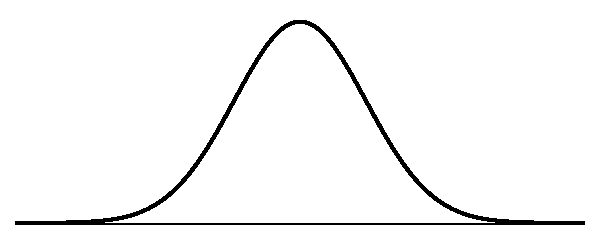
\includegraphics[width=0.6\textwidth]{03/figures/simpleNormal/simpleNormal}
\caption{A normal curve.}
\label{simpleNormal}
\end{figure}

\begin{termBox}{\tBoxTitle{Normal distribution facts}
Many variables are nearly normal, but none are exactly normal. Thus the normal distribution, while not perfect for any single problem, is very useful for a variety of problems. We will use it in data exploration and to solve important problems in statistics.\vspace{0.7mm}}
\end{termBox}

\subsection{Normal distribution model}

The normal distribution model always describes a symmetric, unimodal, bell-shaped curve. However, these curves can look different depending on the details of the model. Specifically, the normal distribution model can be adjusted using two parameters: mean and standard deviation. As you can probably guess, changing the mean shifts the bell curve to the left or right, while changing the standard deviation stretches or constricts the curve. Figure~\ref{twoSampleNormals} shows the normal distribution with mean $0$ and standard deviation $1$ in the left panel and the normal distributions with mean $19$ and standard deviation $4$ in the right panel. Figure~\ref{twoSampleNormalsStacked} shows these distributions on the same axis.

\Comment{added footnote}

\begin{figure}[hht]
\centering
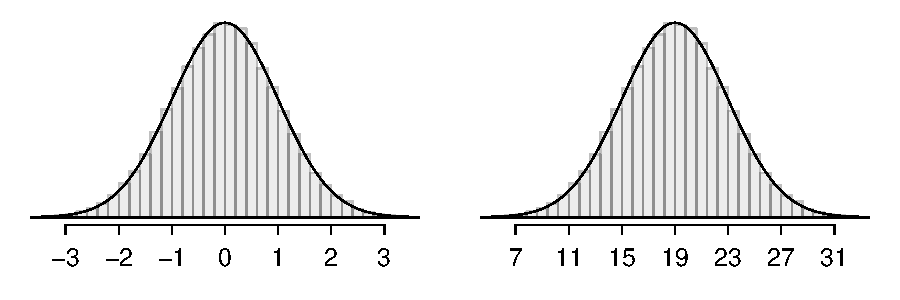
\includegraphics[width=0.9\textwidth]{03/figures/twoSampleNormals/twoSampleNormals}
\caption{Both curves represent the normal distribution, however, they differ in their center and spread. The normal distribution with mean 0 and standard deviation 1 is called the \term{standard normal distribution}.\protect\footnotemark}
\label{twoSampleNormals}
\end{figure}

\footnotetext{The standard normal distribution is described by the density function $f(z) = \frac{1}{{\sqrt {2\pi } }}e^{ - \frac{{z^2 }}{2}}$.  \newline \indent It is a common problem in calculus to show that the integral of this function from $-\infty$ to $+\infty$ equals 1.  }

\begin{figure}[hht]
\centering
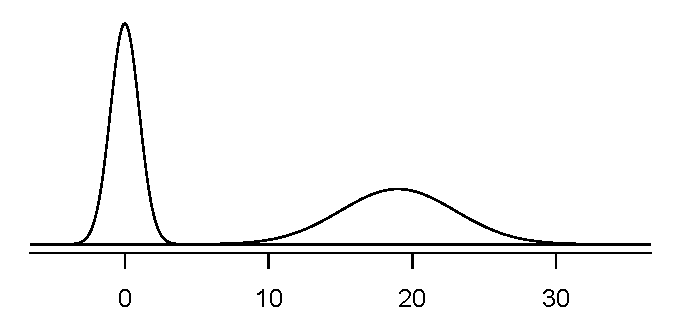
\includegraphics[width=0.62\textwidth]{03/figures/twoSampleNormalsStacked/twoSampleNormalsStacked}
\caption{The normal models shown in Figure~\ref{twoSampleNormals} but plotted together and on the same scale.}
\label{twoSampleNormalsStacked}
\end{figure}

If a normal distribution has mean $\mu$ and standard deviation $\sigma$, we may write the distribution as $N(\mu, \sigma)$\marginpar[\raggedright\vspace{-5mm}

$N(\mu, \sigma)$\vspace{1mm}\\\footnotesize Normal dist.\\with mean $\mu$\\\& st. dev. $\sigma$]{\raggedright\vspace{-5mm}

$N(\mu, \sigma)$\vspace{1mm}\\\footnotesize Normal dist.\\with mean $\mu$\\\& st. dev. $\sigma$}. The two distributions in Figure~\ref{twoSampleNormalsStacked} can be written as
\begin{align*}
N(\mu=0,\sigma=1)\quad\text{and}\quad N(\mu=19,\sigma=4)
\end{align*}
Because the mean and standard deviation describe a normal distribution exactly, they are called the distribution's \termsub{parameters}{parameter}.

\Cut{
\begin{exercise}
Write down the short-hand for a normal distribution with (a)~mean~5 and standard deviation~3, (b)~mean~-100 and standard deviation~10, and (c)~mean~2 and standard deviation~9.\footnote{(a)~$N(\mu=5,\sigma=3)$. (b)~$N(\mu=-100, \sigma=10)$. (c)~$N(\mu=2, \sigma=9)$.}
\end{exercise}
}
\subsection{Standardizing with Z scores}

\Cut{
\begin{example}{Table~\vref{satACTstats} shows the mean and standard deviation for total scores on the SAT and ACT. The distribution of SAT and ACT scores are both nearly normal. Suppose Ann scored 1800 on her SAT and Tom scored 24 on his ACT. Who performed better?}\label{actSAT}
We use the standard deviation as a guide. Ann is 1 standard deviation above average on the SAT: $1500 + 300=1800$. Tom is 0.6 standard deviations above the mean on the ACT: $21+0.6\times 5=24$. In Figure~\ref{satActNormals}, we can see that Ann tends to do better with respect to everyone else than Tom did, so her score was better.
\end{example}

\begin{table}
\centering
\begin{tabular}{l r r}
  \hline
  & SAT & ACT \\
  \hline
Mean \hspace{0.3cm} & 1500 & 21 \\
SD & 300 & 5 \\
   \hline
\end{tabular}
\caption{Mean and standard deviation for the SAT and ACT.}
\label{satACTstats}
\end{table}

\begin{figure}
\centering
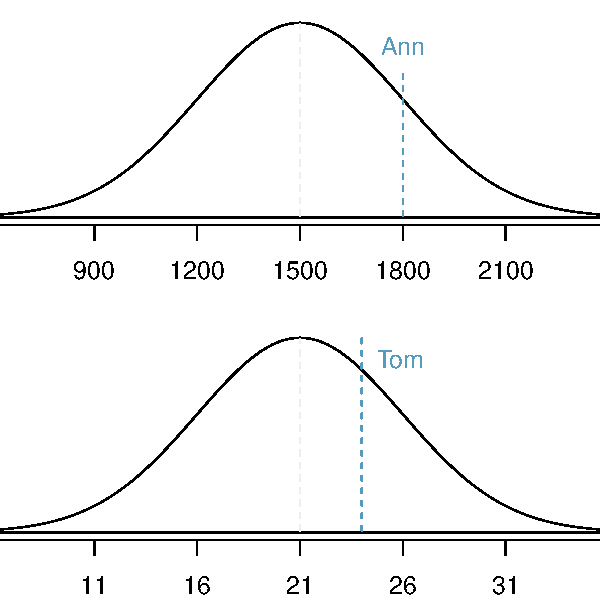
\includegraphics[width=65mm]{03/figures/satActNormals/satActNormals}
\caption{Ann's and Tom's scores shown with the distributions of SAT and ACT scores.}
\label{satActNormals}
\end{figure}

Example~\ref{actSAT} used a standardization technique called a Z score, a method most commonly employed for nearly normal observations but that may be used with any distribution. The \term{Z score}\marginpar[\raggedright\vspace{-3mm}

$Z$\vspace{1mm}\\\footnotesize Z score, the\\standardized\\observation]{\raggedright\vspace{-3mm}

$Z$\vspace{1mm}\\\footnotesize Z score, the\\standardized\\observation}\index{Z@$Z$} of an observation is defined as the number of standard deviations it falls above or below the mean. If the observation is one standard deviation above the mean, its Z score is 1. If it is 1.5 standard deviations \emph{below} the mean, then its Z score is -1.5. If $x$ is an observation from a distribution $N(\mu, \sigma)$, we define the Z score mathematically as
\begin{eqnarray*}
Z = \frac{x-\mu}{\sigma}
\end{eqnarray*}
Using $\mu_{SAT}=1500$, $\sigma_{SAT}=300$, and $x_{Ann}=1800$, we find Ann's Z score:
\begin{eqnarray*}
Z_{Ann} = \frac{x_{Ann} - \mu_{SAT}}{\sigma_{SAT}} = \frac{1800-1500}{300} = 1
\end{eqnarray*}
}

\Add{
\begin{example}{Historical measurements of daily maximum temperature for the month of November are estimated for two cities.\footnote{Data estimated from \urlwofont{http://weatherspark.com} and \urlwofont{http://www.climatestations.com/san-francisco}.}  The summary statistics are as follows.  

\begin{center}	
\begin{tabular}{l l}
San Francisco \hspace{2cm} & London \\
$\mu = 62\degree F$ &  $\mu = 12\degree C$\\
$\sigma= 5\degree F$ &$ \sigma = 2\degree C$.
\end{tabular}
\end{center}

Suppose a particular day in November is 67\degree F in San Francisco and  16\degree C in London.  Which temperature represents a more extreme case?}Because the temperatures are measured in different scales and have different standard deviations, it would not be fair to look at \emph{how many} degrees the values are above average.  67\degree F is 5 degrees above average while 16\degree C is 4 degrees above average, but 67\degree F is 1 \emph{standard deviation} above average while 16\degree C is 2 \emph{standard deviations} above average.  Therefore, 16\degree C represents a more unusual case because, relative to its distribution, it is farther from the mean.
\end{example}

The example above converted the temperatures into \term{standard units} or \term{Z scores}.  A Z score is commonly employed for nearly normal observations but that may be used with any distribution. The \term{Z score}\marginpar[\raggedright\vspace{-3mm}

$Z$\vspace{1mm}\\\footnotesize Z score, the\\standardized\\observation]{\raggedright\vspace{-3mm}

$Z$\vspace{1mm}\\\footnotesize Z score, the\\standardized\\observation}\index{Z@$Z$} of an observation is defined as the number of standard deviations it falls above or below the mean. If the observation is one standard deviation above the mean, its Z score is 1. If it is 1.5 standard deviations \emph{below} the mean, then its Z score is -1.5.

To calculate the Z score for 67\degree F, we do:
\begin{align*}
Z = \frac{x-\mu}{\sigma} = \frac{67-62}{5} = 1
\end{align*}
}

\begin{termBox}{\tBoxTitle{The Z score}
The Z score of an observation is the number of standard deviations it falls above or below the mean. We compute the Z score for an observation $x$ that follows a distribution with mean $\mu$ and standard deviation $\sigma$ using
\begin{eqnarray*}
Z = \frac{x-\mu}{\sigma}
\end{eqnarray*}}
\end{termBox}

\Cut{
\begin{exercise}
Use Tom's ACT score, 24, along with the ACT mean and standard deviation to compute his Z score.\footnote{$Z_{Tom} = \frac{x_{Tom} - \mu_{ACT}}{\sigma_{ACT}} = \frac{24 - 21}{5} = 0.6$}
\end{exercise}
}

Observations above the mean always have positive Z scores while those below the mean have negative Z scores. If an observation is equal to the mean (e.g. SAT score of 1500), then the Z score is $0$.

\Cut{
\begin{exercise}
Let $X$ represent a random variable from $N(\mu=3, \sigma=2)$, and suppose we observe $x=5.19$. (a) Find the Z score of $x$. (b) Use the Z score to determine how many standard deviations above or below the mean $x$ falls.\footnote{(a) Its Z score is given by $Z = \frac{x-\mu}{\sigma} = \frac{5.19 - 3}{2} = 2.19/2 = 1.095$. (b) The observation $x$ is 1.095 standard deviations \emph{above} the mean. We know it must be above the mean since $Z$ is positive.}
\end{exercise}
}

\Add{
\begin{exercise}
Let $X$ represent a random variable with mean $\mu=3$  and standard deviation $\sigma=2$.  Suppose we observe $x=5.19$. (a) Find the Z score of $x$. (b) Use the Z score to determine how many standard deviations above or below the mean $x$ falls.\footnote{(a) Its Z score is given by $Z = \frac{x-\mu}{\sigma} = \frac{5.19 - 3}{2} = 2.19/2 = 1.095$. (b) The observation $x$ is 1.095 standard deviations \emph{above} the mean. We know it must be above the mean since $Z$ is positive.}
\end{exercise}
}

\begin{exercise} \label{headLZScore}
Head lengths of brushtail possums follow a nearly normal distribution with mean 92.6 mm and standard deviation 3.6 mm. Compute the Z scores for possums with head lengths of 95.4 mm and 85.8 mm.\footnote{For $x_1=95.4$ mm: $Z_1 = \frac{x_1 - \mu}{\sigma} = \frac{95.4 - 92.6}{3.6} = 0.78$. For $x_2=85.8$ mm: $Z_2 = \frac{85.8 - 92.6}{3.6} = -1.89$.}
\end{exercise}

We can use Z scores to roughly identify which observations are more unusual than others. One observation $x_1$ is said to be more unusual than another observation $x_2$ if the absolute value of its Z score is larger than the absolute value of the other observation's Z score: $|Z_1| > |Z_2|$. This technique is especially insightful when a distribution is symmetric.

\begin{exercise}
Which of the observations in Guided Practice~\ref{headLZScore} is more unusual?\footnote{Because the \emph{absolute value} of Z score for the second observation is larger than that of the first, the second observation has a more unusual head length.}
\end{exercise}

\Add{
\begin{table}
\centering
\begin{tabular}{l r r}
  \hline
  & SAT & ACT \\
  \hline
Mean \hspace{0.3cm} & 1500 & 21 \\
SD & 300 & 5 \\
   \hline
\end{tabular}
\caption{Mean and standard deviation for the SAT and ACT.}
\label{satACTstats}
\end{table}

\begin{example}{Table~\vref{satACTstats} shows the mean and standard deviation for total scores on the SAT and ACT. \Cut{The distribution of SAT and ACT scores are both nearly normal.} Suppose Ann scored 1800 on her SAT and Tom scored 24 on his ACT. Who performed better?}\label{actSAT}
We cannot compare their scores directly; we must convert them to standard units.   
\begin{align*}
Z_{Ann} &= \frac{x_{Ann} - \mu_{SAT}}{\sigma_{SAT}} = \frac{1800-1500}{300} = 1 \\   
Z_{Tom} &= \frac{x_{Tom} - \mu_{ACT}}{\sigma_{ACT}} = \frac{24-21}{5} = 0.6
\end{align*}
Ann is 1 standard deviation above average on the SAT and Tom is 0.6 standard deviations above average on the ACT, so Ann performed better with respect to the other test takers than Tom.  
\end{example}
}

\subsection{68-95-99.7 rule}
\Comment{this subsection moved here - was after normal table section}

Here, we present a useful rule of thumb for the probability of falling within 1, 2, and 3 standard deviations of the mean in the normal distribution. This will be useful in a wide range of practical settings, especially when trying to make a quick estimate without a calculator or Z table.

\Comment{added ``The normal curve is the basis for the Empirical Rule we encountered in Chapter 2. The closer a distribution is to the normal curve, the more accurate the 68-95-99.7 rule will be" to figure caption.
}
\begin{figure}[hht]
\centering
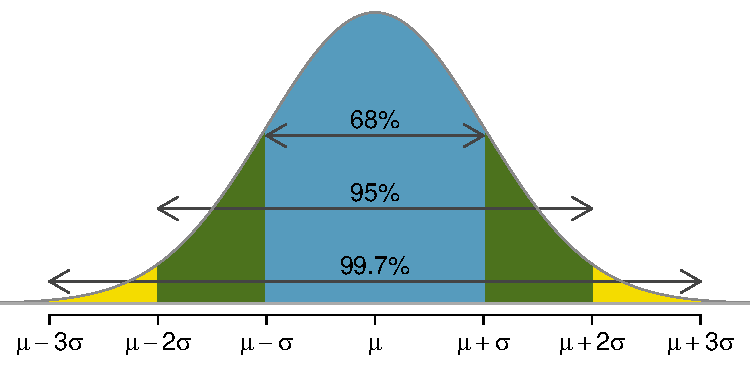
\includegraphics[height=1.9in]{03/figures/6895997/6895997}
\caption{Probabilities for falling within 1, 2, and 3 standard deviations of the mean in a normal distribution. The normal curve is the basis for the Empirical Rule we encountered in Chapter 2. The closer a distribution is to the normal curve, the more accurate the 68-95-99.7 rule will be.}
\label{6895997}
\end{figure}

\begin{exercise}
Use the Z table to confirm that about 68\%, 95\%, and 99.7\% of observations fall within 1, 2, and 3, standard deviations of the mean in the normal distribution, respectively. For instance, first find the area that falls between $Z=-1$ and $Z=1$, which should have an area of about 0.68. Similarly there should be an area of about 0.95 between $Z=-2$ and $Z=2$.\footnote{First draw the pictures. To find the area between $Z=-1$ and $Z=1$, use the normal probability table to determine the areas below $Z=-1$ and above $Z=1$. Next verify the area between $Z=-1$ and $Z=1$ is about 0.68. Repeat this for $Z=-2$ to $Z=2$ and also for $Z=-3$ to $Z=3$.}
\end{exercise}

It is possible for a normal random variable to fall 4,~5, or~even more standard deviations from the mean. However, these occurrences are very rare if the data are nearly normal. The probability of being further than 4 standard deviations from the mean is about 1-in-30,000. For 5 and 6 standard deviations, it is about 1-in-3.5 million and 1-in-1 billion, respectively.

\begin{exercise}
SAT scores closely follow the normal model with mean $\mu = 1500$ and standard deviation $\sigma = 300$. (a) About what percent of test takers score 900 to 2100? (b) What percent score between 1500 and 2100?\footnote{(a) 900 and 2100 represent two standard deviations above and below the mean, which means about 95\% of test takers will score between 900 and 2100. (b)~Since the normal model is symmetric, then half of the test takers from part~(a) ($\frac{95\%}{2} = 47.5\%$ of all test takers) will score 900 to 1500 while 47.5\% score between 1500 and 2100.}
\end{exercise}


%\begin{exercise} \label{email_num_char_ZScore}
%The variable \var{num\_\hspace{0.3mm}char} from the \data{email} data set describes the number of characters in nearly 4,000 emails. The distribution has mean 10,476 and standard deviation 14,383. Identify the Z scores for $\var{num\_\hspace{0.3mm}char}_{36}=13,788$ mm and $\var{num\_\hspace{0.3mm}char}_{79}=3,485$, which correspond to the $36^{th}$ and $76^{th}$ emails in the data set.\footnote{$Z_{36} = \frac{13,788 - 10,476}{14,383} = 0.23$, $Z_{79} = \frac{3,485 - 10,476}{14,383} = -0.49$}
%\end{exercise}

%\begin{exercise}
%Which of the observations in Guided Practice~\ref{email_num_char_ZScore} is more unusual?\footnote{In Guided Practice~\ref{email_num_char_ZScore}, $Z_{36} = 0.23$ and $Z_{79}=-0.49$. Because the \emph{absolute value} of $Z_{79}$ is larger than $Z_{36}$, case 79 appears to have a more unusual number of email characters.}
%\end{exercise}

\subsection{Normal probability table}

\begin{example}{Ann from Example~\ref{actSAT} earned a score of 1800 on her SAT with a corresponding $Z=1$. She would like to know what percentile she falls in among all SAT test-takers.}
Ann's \term{percentile} is the percentage of people who earned a lower SAT score than Ann. \Add{In the section on box plots and quartiles, we learned how to find the 25th, 50th, and 75th percentiles of a distribution.  To find Ann's exact percentile, we would have to know how many people scored less than her and how many total people took the test, information that is not readily available.  However, because the distribution of SAT score is approximately normal, we can estimate this answer using normal approximation.}  We shade the area representing those individuals in Figure~\ref{satBelow1800}. The total area under the normal curve is always equal to 1, and the proportion of people who scored below Ann on the SAT is \Add{approximately} equal to the \emph{area} shaded in Figure~\ref{satBelow1800}: 0.8413. In other words, Ann is in the $84^{th}$ percentile of SAT takers.
\end{example}

\Comment{Use/adapt first figure rather than second?}

\begin{figure}
\centering
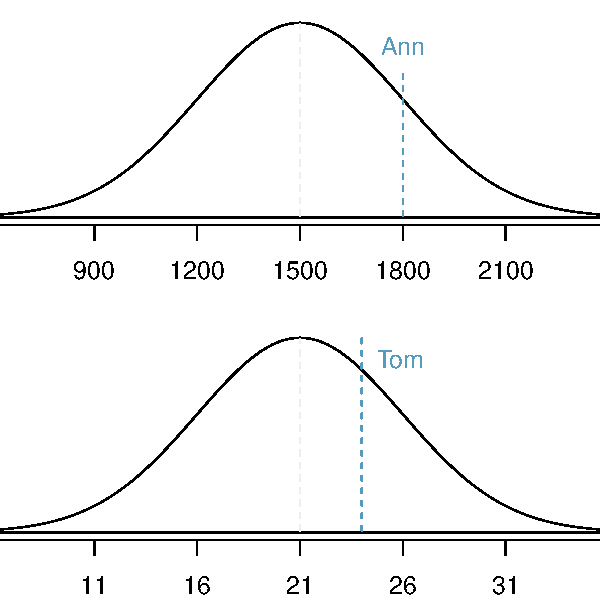
\includegraphics[width=65mm]{03/figures/satActNormals/satActNormals}
\caption{Ann's and Tom's scores shown with the distributions of SAT and ACT scores.}
\label{satActNormals}
\end{figure}


\begin{figure}[htb]
   \centering
   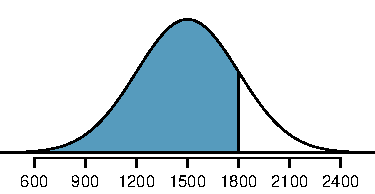
\includegraphics[height=1.5in]{03/figures/satBelow1800/satBelow1800}
   \caption{The normal model for SAT scores, shading the area of those individuals who scored below Ann.}
   \label{satBelow1800}
\end{figure}

\Add{In order to find the area under the curve to left of Ann's score, we use a \term{standard normal probability table}, or \term{normal probability table} for short.  Because these tables use Z scores, we must first convert Ann's score to a Z score.  Using the normal probability table we can identify the percentile that corresponds to a Z score (and vice versa).  Statistical software can also be used.}  \Cut{We can use the normal model to find percentiles. A \term{normal probability table}, which lists Z scores and corresponding percentiles, can be used to identify a percentile based on the Z score (and vice versa). Statistical software can also be used.}

A normal probability table is given in Appendix~\vref{normalProbabilityTable} and abbreviated in Table~\ref{zTableShort}. We use this table to identify the percentile corresponding to any particular Z score. For instance, the percentile of $Z=0.43$ is shown in row $0.4$ and column $0.03$ in Table~\ref{zTableShort}: 0.6664, or the $66.64^{th}$ percentile. Generally, we round $Z$ to two decimals, identify the proper row in the normal probability table up through the first decimal, and then determine the column representing the second decimal value. The intersection of this row and column is the percentile of the observation.

\begin{figure}
\centering
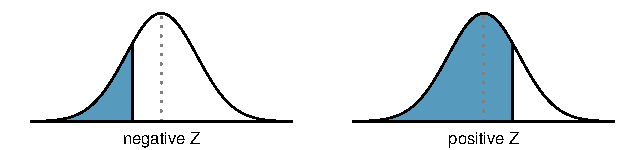
\includegraphics[width=0.8\textwidth]{03/figures/normalTails/normalTails}
\caption{The area to the left of $Z$ represents the percentile of the observation.}
\label{normalTails}
\end{figure}

\begin{table}
\centering
\begin{tabular}{c | rrrrr | rrrrr |}
  \cline{2-11}
&&&& \multicolumn{4}{c}{Second decimal place of $Z$} &&& \\
  \cline{2-11}
$Z$ & 0.00 & 0.01 & 0.02 & \highlightT{0.03} & \highlightO{0.04} & 0.05 & 0.06 & 0.07 & 0.08 & 0.09 \\
  \hline
  \hline
0.0 & \scriptsize{0.5000} & \scriptsize{0.5040} & \scriptsize{0.5080} & \scriptsize{0.5120} & \scriptsize{0.5160} & \scriptsize{0.5199} & \scriptsize{0.5239} & \scriptsize{0.5279} & \scriptsize{0.5319} & \scriptsize{0.5359} \\
  0.1 & \scriptsize{0.5398} & \scriptsize{0.5438} & \scriptsize{0.5478} & \scriptsize{0.5517} & \scriptsize{0.5557} & \scriptsize{0.5596} & \scriptsize{0.5636} & \scriptsize{0.5675} & \scriptsize{0.5714} & \scriptsize{0.5753} \\
  0.2 & \scriptsize{0.5793} & \scriptsize{0.5832} & \scriptsize{0.5871} & \scriptsize{0.5910} & \scriptsize{0.5948} & \scriptsize{0.5987} & \scriptsize{0.6026} & \scriptsize{0.6064} & \scriptsize{0.6103} & \scriptsize{0.6141} \\
%  May comment out 0.0-0.2 to make extra space. Then insert the following line:
%  $\vdots$ &   $\vdots$ &   $\vdots$ &   $\vdots$ &   $\vdots$ &   $\vdots$ &   $\vdots$ &   $\vdots$ &   $\vdots$ &   $\vdots$ &   $\vdots$ \\
  0.3 & \scriptsize{0.6179} & \scriptsize{0.6217} & \scriptsize{0.6255} & \scriptsize{0.6293} & \scriptsize{0.6331} & \scriptsize{0.6368} & \scriptsize{0.6406} & \scriptsize{0.6443} & \scriptsize{0.6480} & \scriptsize{0.6517} \\
\highlightT{0.4} & \scriptsize{0.6554} & \scriptsize{0.6591} & \scriptsize{0.6628} & \highlightT{\scriptsize{0.6664}} & \scriptsize{0.6700} & \scriptsize{0.6736} & \scriptsize{0.6772} & \scriptsize{0.6808} & \scriptsize{0.6844} & \scriptsize{0.6879} \\
  \hline
  0.5 & \scriptsize{0.6915} & \scriptsize{0.6950} & \scriptsize{0.6985} & \scriptsize{0.7019} & \scriptsize{0.7054} & \scriptsize{0.7088} & \scriptsize{0.7123} & \scriptsize{0.7157} & \scriptsize{0.7190} & \scriptsize{0.7224} \\
  0.6 & \scriptsize{0.7257} & \scriptsize{0.7291} & \scriptsize{0.7324} & \scriptsize{0.7357} & \scriptsize{0.7389} & \scriptsize{0.7422} & \scriptsize{0.7454} & \scriptsize{0.7486} & \scriptsize{0.7517} & \scriptsize{0.7549} \\
  0.7 & \scriptsize{0.7580} & \scriptsize{0.7611} & \scriptsize{0.7642} & \scriptsize{0.7673} & \scriptsize{0.7704} & \scriptsize{0.7734} & \scriptsize{0.7764} & \scriptsize{0.7794} & \scriptsize{0.7823} & \scriptsize{0.7852} \\
\highlightO{0.8} & \scriptsize{0.7881} & \scriptsize{0.7910} & \scriptsize{0.7939} & \scriptsize{0.7967} & \highlightO{\scriptsize{0.7995}} & \scriptsize{0.8023} & \scriptsize{0.8051} & \scriptsize{0.8078} & \scriptsize{0.8106} & \scriptsize{0.8133} \\
  0.9 & \scriptsize{0.8159} & \scriptsize{0.8186} & \scriptsize{0.8212} & \scriptsize{0.8238} & \scriptsize{0.8264} & \scriptsize{0.8289} & \scriptsize{0.8315} & \scriptsize{0.8340} & \scriptsize{0.8365} & \scriptsize{0.8389} \\
  \hline
  \hline
  1.0 & \scriptsize{0.8413} & \scriptsize{0.8438} & \scriptsize{0.8461} & \scriptsize{0.8485} & \scriptsize{0.8508} & \scriptsize{0.8531} & \scriptsize{0.8554} & \scriptsize{0.8577} & \scriptsize{0.8599} & \scriptsize{0.8621} \\
  1.1 & \scriptsize{0.8643} & \scriptsize{0.8665} & \scriptsize{0.8686} & \scriptsize{0.8708} & \scriptsize{0.8729} & \scriptsize{0.8749} & \scriptsize{0.8770} & \scriptsize{0.8790} & \scriptsize{0.8810} & \scriptsize{0.8830} \\
  $\vdots$ &   $\vdots$ &   $\vdots$ &   $\vdots$ &   $\vdots$ &   $\vdots$ &   $\vdots$ &   $\vdots$ &   $\vdots$ &   $\vdots$ &   $\vdots$ \\
   \hline
\end{tabular}
\caption{A section of the normal probability table. The percentile for a normal random variable with $Z=0.43$ has been \highlightT{highlighted}, and the percentile closest to 0.8000 has also been \highlightO{highlighted}.}
\label{zTableShort}
\end{table}

We can also find the Z score associated with a percentile. For example, to identify Z for the $80^{th}$ percentile, we look for the value closest to 0.8000 in the middle portion of the table: 0.7995. We determine the Z score for the $80^{th}$ percentile by combining the row and column Z values: 0.84.

\begin{exercise}
Determine the proportion of SAT test takers who scored better than Ann on the SAT.\footnote{If 84\% had lower scores than Ann, the number of people who had better scores must be 16\%. (Generally ties are ignored when the normal model, or any other continuous distribution, is used.)}
\end{exercise}

\subsection{Normal probability examples}

Cumulative SAT scores are approximated well by a normal model, $N(\mu=1500, \sigma=300)$.


\begin{example}{\Cut{Shannon is a randomly selected SAT taker, and nothing is known about Shannon's SAT aptitude. What is the probability Shannon scores at least 1630 on her SATs?}\Add{What is the probability that a randomly selected SAT taker scores at least 1630 on the SAT?}}\label{satAbove1630Exam}
\Add{The probability that a randomly selected SAT taker scores at least 1630 on the SAT is equivalent to the \emph{proportion} of all SAT takers that score at least 1630 on the SAT.} First, always draw and label a picture of the normal distribution. (Drawings need not be exact to be useful.) We are interested in the \Cut{chance she scores} \Add{probability that a randomly selected score will be} above 1630, so we shade this upper tail:
\begin{center}
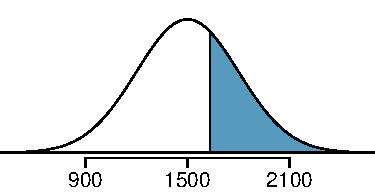
\includegraphics[height=0.9in]{03/figures/satAbove1630/satAbove1630}
\end{center}
The picture shows the mean and the values at 2 standard deviations above and below the mean. The simplest way to find the shaded area under the curve makes use of the Z score of the cutoff value. With $\mu=1500$, $\sigma=300$, and the cutoff value $x=1630$, the Z score is computed as
\begin{eqnarray*}
Z = \frac{x - \mu}{\sigma} = \frac{1630 - 1500}{300} = \frac{130}{300} = 0.43
\end{eqnarray*}
We look up the percentile of $Z=0.43$ in the normal probability table shown in Table~\ref{zTableShort} or in Appendix~\vref{normalProbabilityTable}, which yields 0.6664. However, the percentile describes those who had a Z score \emph{lower} than 0.43. To find the area \emph{above} $Z=0.43$, we compute one minus the area of the lower tail:
\begin{center}
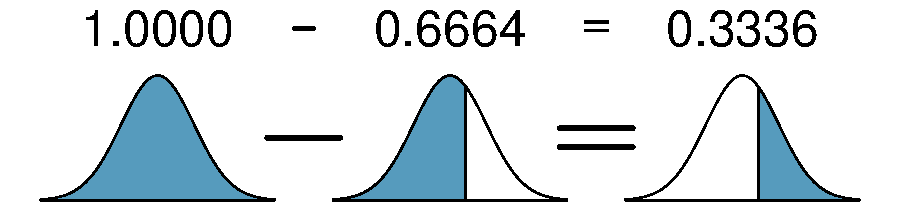
\includegraphics[height=0.8in]{03/figures/subtractingArea/subtractingArea}
\end{center}
The probability \Cut{Shannon scores} \Add{that a randomly selected score is} at least 1630 on the SAT is 0.3336.
\end{example}

\begin{tipBox}{\tipBoxTitle{always draw a picture first, and find the Z score second}
For any normal probability situation, \emph{always always always} draw and label the normal curve and shade the area of interest first. The picture will provide an estimate of the probability. \vspace{3mm}

After drawing a figure to represent the situation, identify the Z score for the observation of interest.\vspace{1mm}}
\end{tipBox}

\begin{exercise}
\Cut{If the probability of Shannon scoring at least 1630 is 0.3336, then what is the probability she scores less than 1630?} \Add{If the probability that a randomly selected score is at least 1630, what is the probability that the score is less than 1630?} Draw the normal curve representing this exercise, shading the lower region instead of the upper one.\footnote{We found the probability in Example~\ref{satAbove1630Exam}: 0.6664. A picture for this exercise is represented by the shaded area below ``0.6664'' in Example~\ref{satAbove1630Exam}.}
\end{exercise}

\begin{example}{Edward earned a 1400 on his SAT. What is his percentile?} \label{edwardSatBelow1400}
First, a picture is needed. Edward's percentile is the proportion of people who do not get as high as a 1400. These are the scores to the left of 1400.
\begin{center}
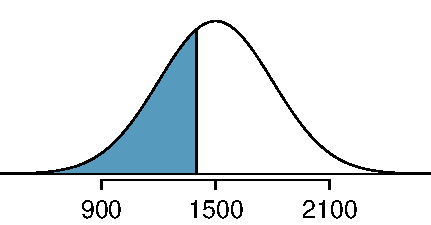
\includegraphics[height=22mm]{03/figures/satBelow1400/satBelow1400}
\end{center}
Identifying the mean $\mu=1500$, the standard deviation $\sigma=300$, and the cutoff for the tail area $x=1400$ makes it easy to compute the Z score:
\begin{eqnarray*}
Z = \frac{x - \mu}{\sigma} = \frac{1400 - 1500}{300} = -0.33
\end{eqnarray*}
Using the normal probability table, identify the row of $-0.3$ and column of $0.03$, which corresponds to the probability $0.3707$. Edward is at the $37^{th}$ percentile.
\end{example}

\begin{exercise}
Use the results of Example~\ref{edwardSatBelow1400} to compute the proportion of SAT takers who did better than Edward. Also draw a new picture.\footnote{If Edward did better than 37\% of SAT takers, then about 63\% must have done better than him. \\
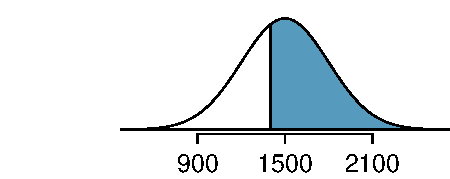
\includegraphics[height=12mm]{03/figures/satBelow1400/satAbove1400}}
\end{exercise}

\begin{tipBox}{\tipBoxTitle{areas to the right}
The normal probability table in most books gives the area to the left. If you would like the area to the right, first find the area to the left and then subtract this amount from~one.}
\end{tipBox}

\Add{
The last several problems have focused on finding the probability or percentile for a particular observation. It is also possible to identify the value corresponding to a particular percentile.

\begin{example}{Larry believes he can get into his preferred college if he scores at least in the 80th percentile on the SAT. What score should he aim for?}Here, we are given a percentile rather than a Z score, so we work backwards.  As always, first draw the picture. \Comment{TODO(David) insert picture}
We want to find the observation that corresponds to the 80th percentile.  First, we find the Z score associated with the 80th percentile using the normal probability table.  Looking at Table~\ref{zTableShort}., we look for the number closest to 0.80 \emph{inside} the table.  The closest number we find is 0.7995 (highlighted in blue).  0.7995 falls on row 0.8 and column 0.04, therefore it corresponds to a Z score of 0.84.  In any normal distribution, a value with a Z score of 0.84 will be at the 80th percentile.  Once we have the Z score, we work backwards to find x.

\begin{align*}
Z &= \frac{x-\mu}{\sigma} \\
0.84 &= \frac{x-1500}{300} \\
(.84)(300)+1500 &= x \\
x& = 1752
\end{align*}

The 80th percentile on the SAT corresponds to a score of 1752.
\end{example}

\begin{exercise}Mary scored at the 72nd percentile on the SAT.  What was her SAT score?\footnote{The Z score corresponding to 0.7190 (the closest number inside the table to 0.72) is 0.58. \newline \indent $0.58 = \frac{x-1500}{300}$ , so $x = 1674$.   Mary scored 1674.}
\end{exercise}
}

\Comment{added caution box}

\begin{caution}{If the data are not nearly normal, don't use a normal table}{
Before using the normal table, verify that the data or distribution is approximately normal.  If it is not, the normal table will give incorrect results.  Also, all answers based on normal approximations are approximations and are not exact.}
\end{caution}

\Cut{
\begin{exercise}
Stuart earned an SAT score of 2100. Draw a picture for each part. (a)~What is his percentile? (b)~What percent of SAT takers did better than Stuart?\footnote{Numerical answers: (a) 0.9772. (b) 0.0228.}
\end{exercise}

Based on a sample of 100 men,\footnote{This sample was taken from the USDA Food Commodity Intake Database.} the heights of male adults between the ages 20 and 62 in the US is nearly normal with mean 70.0'' and standard deviation 3.3''.

\begin{exercise}
Mike is 5'7'' and Jim is 6'4''. (a) What is Mike's height percentile? (b) What is Jim's height percentile? Also draw one picture for each part.\footnote{First put the heights into inches: 67 and 76 inches. Figures are shown below. (a) $Z_{Mike} = \frac{67 - 70}{3.3} = -0.91\ \to\ 0.1814$. (b) $Z_{Jim} = \frac{76 - 70}{3.3} = 1.82\ \to\ 0.9656$. \\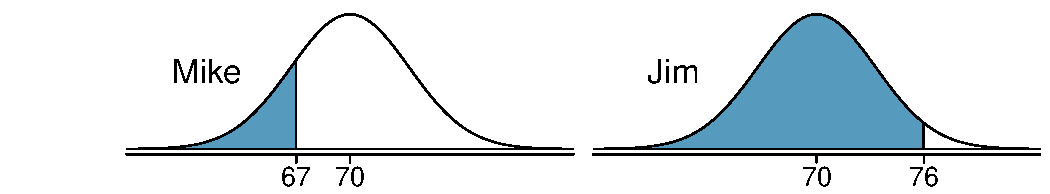
\includegraphics[height=12mm]{03/figures/mikeAndJimPercentiles/mikeAndJimPercentiles}}
\end{exercise}


The last several problems have focused on finding the probability or percentile for a particular observation. What if you would like to know the observation corresponding to a particular percentile?

\begin{example}{Erik's height is at the $40^{th}$ percentile. How tall is he?}\label{normalExam40Perc}
As always, first draw the picture.\vspace{-1mm}
\begin{center}
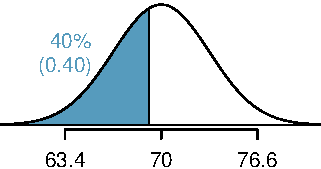
\includegraphics[height=22mm]{03/figures/height40Perc/height40Perc}\vspace{-1mm}
\end{center}
In this case, the lower tail probability is known (0.40), which can be shaded on the diagram. We want to find the observation that corresponds to this value. As a first step in this direction, we determine the Z score associated with the $40^{th}$ percentile.

Because the percentile is below 50\%, we know $Z$ will be negative. Looking in the negative part of the normal probability table, we search for the probability \emph{inside} the table closest to 0.4000. We find that 0.4000 falls in row $-0.2$ and between columns $0.05$ and $0.06$. Since it falls closer to $0.05$, we take this one: $Z=-0.25$.

Knowing $Z_{Erik}=-0.25$ and the population parameters $\mu=70$ and $\sigma=3.3$ inches, the Z score formula can be set up to determine Erik's unknown height, labeled $x_{Erik}$:
\begin{eqnarray*}
-0.25 = Z_{Erik} = \frac{x_{Erik} - \mu}{\sigma} = \frac{x_{Erik} - 70}{3.3}
\end{eqnarray*}
Solving for $x_{Erik}$ yields the height 69.18 inches. That is, Erik is about 5'9'' (this is notation for 5-feet, 9-inches).
\end{example}


\begin{example}{What is the adult male height at the $82^{nd}$ percentile?}
Again, we draw the figure first.\vspace{-1mm}
\begin{center}
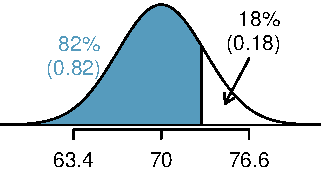
\includegraphics[height=22mm]{03/figures/height82Perc/height82Perc}\vspace{-1mm}
\end{center}
Next, we want to find the Z score at the $82^{nd}$ percentile, which will be a positive value. Looking in the Z table, we find $Z$ falls in row $0.9$ and the nearest column is $0.02$, i.e. $Z=0.92$. Finally, the height $x$ is found using the Z score formula with the known mean $\mu$, standard deviation $\sigma$, and Z score $Z=0.92$:
\begin{eqnarray*}
0.92 = Z = \frac{x-\mu}{\sigma} = \frac{x - 70}{3.3}
\end{eqnarray*}
This yields 73.04 inches or about 6'1'' as the height at the $82^{nd}$ percentile.
\end{example}

\begin{exercise}
(a) What is the $95^{th}$ percentile for SAT scores? (b) What is the $97.5^{th}$ percentile of the male heights? As always with normal probability problems, first draw a picture.\footnote{Remember: draw a picture first, then find the Z score. (We leave the pictures to you.) The Z score can be found by using the percentiles and the normal probability table. (a) We look for 0.95 in the probability portion (middle part) of the normal probability table, which leads us to row 1.6 and (about) column 0.05, i.e. $Z_{95}=1.65$. Knowing $Z_{95}=1.65$, $\mu = 1500$, and $\sigma = 300$, we setup the Z score formula: $1.65 = \frac{x_{95} - 1500}{300}$. We solve for $x_{95}$: $x_{95} = 1995$. (b) Similarly, we find $Z_{97.5} = 1.96$, again setup the Z score formula for the heights, and calculate $x_{97.5} = 76.5$.}
\end{exercise}

\begin{exercise}\label{more74Less69}
(a)~What is the probability that a randomly selected male adult is at least 6'2'' (74 inches)? (b)~What is the probability that a male adult is shorter than 5'9'' (69 inches)?\footnote{Numerical answers: (a) 0.1131. (b) 0.3821.}
\end{exercise}

\begin{example}{What is the probability that a random adult male is between 5'9'' and 6'2''?}
These heights correspond to 69 inches and 74 inches. First, draw the figure. The area of interest is no longer an upper or lower tail.
\begin{center}
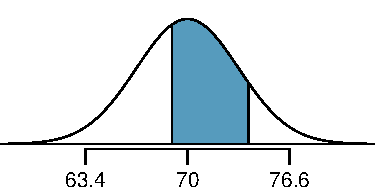
\includegraphics[height=0.85in]{03/figures/between59And62/between59And62}
\end{center}
The total area under the curve is~1. If we find the area of the two tails that are not shaded (from Guided Practice~\ref{more74Less69}, these areas are $0.3821$ and $0.1131$), then we can find the middle area:
\begin{center}
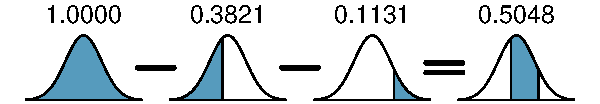
\includegraphics[height=0.65in]{03/figures/subtracting2Areas/subtracting2Areas}
\end{center}
That is, the probability of being between 5'9'' and 6'2'' is 0.5048.
\end{example}

\begin{exercise}
What percent of SAT takers get between 1500 and 2000?\footnote{This is an abbreviated solution. (Be sure to draw a figure!) First find the percent who get below 1500 and the percent that get above 2000: $Z_{1500} = 0.00 \to 0.5000$ (area below), $Z_{2000} = 1.67 \to 0.0475$ (area above). Final answer: $1.0000-0.5000 - 0.0475 = 0.4525$.}
\end{exercise}

\begin{exercise}
What percent of adult males are between 5'5'' and 5'7''?\footnote{5'5'' is 65 inches. 5'7'' is 67 inches. Numerical solution: $1.000 - 0.0649 - 0.8183 = 0.1168$, i.e. 11.68\%.}
\end{exercise}
}


\subsection{Calculator: finding normal probabilities}
\label{TInormal}

\Comment{TODO(David) insert video icon}  

\begin{termBox}{\tBoxTitle{TI calculator:  1.  Finding areas under normal curve}Use \textbf{2ND VARS, normalcdf} to find an area/proportion/probability to the left or right of a Z score or between two Z scores.
\begin{enumerate}
\item Choose 2ND VARS (i.e. DISTR).
\item Choose 2:normalcdf.
\item Enter the Z scores that correspond to the lower (left) and upper (right) bounds.
\item Leave $\mu$ as 0 and $\sigma$ as 1.
\item Down arrow, choose Paste, and hit ENTER.
\newline
\begin{itemize}
\item[TI-83: ] Do steps 1 - 2, then enter the lower bound and upper bound separated by a comma, e.g. normalcdf(2, 5), and hit ENTER.
\end{itemize}
\end{enumerate}
}
\end{termBox}

\begin{example}{Use a calculator to determine what percentile corresponds to a Z score of 1.5.}To find areas under the normal curve on a calculator, we must identify a lower bound and an upper bound.  Always first sketch a graph.  To find a percentile we need the area to the \emph{left} of the Z score.  Theoretically, we want all of the area in the left tail, so the left endpoint should be -$\infty$.  However, the area under the curve quickly becomes negligible (recall that a Z score of -3 is very unlikely).  We will use -5 as the lower bound when there is no given lower bound, but any other negative number smaller than this is also acceptable.\footnote{normalcdf gives the result without drawing the graph.  To draw the graph, do 2nd VARS, DRAW, 1:ShadeNorm.  However, beware of errors caused by other plots that might interfere with this plot.}  Doing 2nd VARS, 2:normalcdf, and using a lower bound of -5 and an upper bound of 1.5, we get $P(Z < 1.5) = 0.933$.
\end{example}

\begin{exercise}Find the area under the the normal curve to right of $Z=2$. \footnote{Now we want to shade to the right.  Therefore our lower bound will be 2 and the upper bound will be +5.  We get $P(Z > 2) = 0.023$.}
\end{exercise}

\begin{exercise}Find the area under the the normal curve between -1.5 and 1.5.  \footnote{Here we are given both the lower and the upper bound.  Lower bound is -1.5 and upper bound is 1.5.  The area under the normal curve between -15 and 1.5 = $P(-1.5 < Z < 1.5) = 0.866$.}
\end{exercise}

\begin{termBox}{\tBoxTitle{TI calculator:  2. Find a Z score that corresponds to a percentile}
Use \textbf{2ND VARS, invNorm} to find the Z score that corresponds to a given percentile.
\begin{enumerate}
\item Choose 2ND VARS (i.e. DISTR).
\item Choose 3:invNorm.
\item Let Area be the percentile as a decimal (the area to the left of desired Z score).
\item Leave $\mu$ as 0 and $\sigma$ as 1.
\item Down arrow, choose Paste, and hit ENTER.
\newline
\begin{itemize}
\item[TI-83: ] Do steps 1 - 2, then enter the percentile as a decimal, e.g. invNorm(.40), then hit ENTER.
\end{itemize}
\end{enumerate}
}
\end{termBox}

\begin{example}{Use a calculator to find the Z score that corresponds to the 40th percentile.}Letting Area be 0.40, a calculator gives -0.253. This means that $Z = -0.253$ corresponds to the 40th percentile, that~is, $P(Z < -0.253) = 0.40$.
\end{example}

\begin{exercise}Find the Z score such that 20 percent of the area is to the right of that Z score.\footnote{If 20\% of the area is the right, then 80\% of the area is to the left.  Letting area be 0.80, we get $Z = 0.841$.}
\end{exercise}
Male
	
	

n=23419
	
3376=7.44lbs (603.33=1.33)

	

\begin{example}{In a large study of birth weight of newborns, the weights of 23,419 newborn boys were recorded.\footnote{\urlwofont{http://www.biomedcentral.com/1471-2393/8/5}}The distribution of weights was approximately normal with a mean of 7.44 lbs (3376 grams) and a standard deviation of 1.33 lbs (603 grams).  The government classifies a newborn as having low birth weight if the weight is less than 5.5 pounds.  What percent of these newborns were of low birth weight?}First we will find a Z score, then we will need an area under the normal curve so we will use ShadeNorm with a lower bound of -5.  The upper bound will be the Z score that we calculate.  There is no need to write calculator commands on your paper.  Instead, continue to use standard statistical notation.  
\begin{align*}
Z&=\frac{5.5-7.44}{1.33}\\
&=-1.49\\
P(Z < -1.49) &= 0.068
\end{align*}
Approximately 6.8\% of the newborns were of low birth weight.
\end{example}

\begin{exercise}Approximately what percent of these babies weighed greater than 10 pounds?\footnote{$Z=\frac{10-7.44}{1.33}=1.925$ Using a lower bound of 2 and an upper bound of 5 we get $P(Z  > 1.925) = 0.027$.  Appoximately 2.7\% of the newborns weighed over 10 pounds.}
\end{exercise}

\begin{exercise}Approximately \emph{how many} of these newborns weighed greater than 10 pounds?\footnote{Appoximately 2.7\% of the newborns weighed over 10 pounds.  Because there were 23,419 of them, 0.027(23419)$\approx$ 632 weighed greater than 10 pounds. }
\end{exercise}

\begin{exercise}How much would a newborn have to weigh in order to be at the 90th percentile among this group?\footnote{Because we have the percentile this is the inverse problem.  To get the $Z$ score we do invNorm of $.90$ and we get $Z =  1.28$.  Then we solve for x using $1.28={x - 7.44}{1.33}$ and we get $x = 9.15$.  To be at the 90th percentile among this group a newborn would have to weigh 9.15 pounds.}
\end{exercise}

\subsection{Normal approximation for sums of random variables}
\label{normapproxsumrv}

We have seen that many distributions are approximately normal.  The sum and the difference of normally distributed variables is also normal.  While we cannot prove this here, the usefulness of it is seen in the following example.

\begin{example}{Three friends are playing a cooperative video game in which they have to complete a puzzle as fast as possible.  Assume that the individual times of the 3 friends are independent of each other. The individual times of the friends in similar puzzles are approximately normally distributed with the following means and standard deviations. 
\begin{center}
\begin{tabular}{lrr}
& Mean &  SD \\
Friend 1 	& 5.6 & 0.11  \\
Friend 2 	& 5.8  & 0.13 \\
Friend 3 	& 6.1  & 0.12  
\end{tabular}
\end{center}
To advance to the next level of the game, the friends' total time must not exceed 17.1 minutes.  What is the probability that they will advance to the next level?
}
Because each friend's time is approximately normally distributed, the \emph{sum} of their times is also approximately normally distributed.  We will do a normal approximation, but first we need to find the mean and standard deviation of the \emph{sum}.  We learned how to do this in the section Random Variables.  Let the three friends be called X, Y, Z.  We want $P(X+Y+Z < 17.1)$. The mean of the sum of X, Y, and Z is given by:
\begin{align*}
\mu_{X+Y+Z} &= E(X+Y+Z)  \\
&= E(X) + E(Y) + E(Z)\\
&=4.6+4.8+4.5 \\
&=17.5
\end{align*}
The standard deviation is given by:
\begin{align*}
SD_{X+Y+Z}&= \sqrt{(SD_X)^2+(SD_Y)^2 + (SD_Z)^2} \\
&= \sqrt{(0.11)^2+(0.13)^2+(0.12)^2} \\
&=0.208
\end{align*}
Now we can find the Z score.  
\begin{align*}
Z &= \frac{x_{sum}-\mu_{sum}}{\sigma_{sum}} \\
&=\frac{17.1-17.5}{.208} \\
&=-1.92
\end{align*}
Finally, we want the probability that the sum is less than 17.5 so we shade to the left of the corresponding Z score of -1.92.  Using the normal table or a calculator we get:
\begin{align*}
P(Z < -1.92) = 0.027
\end{align*}
There is a 2.7\% chance that the friends will advance to the next level.
\end{example}

\begin{exercise}What is the probability that Friend 2 will complete the puzzle with a faster time than Friend 1?  Hint:  find $P(Y < X)$, or $P(Y - X < 0)$.\footnote{First find the mean and standard deviation of $Y - X$.  

The mean of $Y - X$ is $\mu_{Y-X} = 5.8 - 5.6 =  0.2$.  

The standard deviation is  $SD_{Y-X}=\sqrt{(0.13)^2+(0.11)^2}=0.170$.  

$Z=\frac{0-0.2}{0.170}=-1.18$.  

$P(Z < -1.18)= .119$.  

There is an 11.9\% chance that Friend 2 will complete the puzzle with a faster time than Friend 1.}
\end{exercise}


%_________________
\section{Evaluating the normal approximation}
\label{assessingNormal}

Many processes can be well approximated by the normal distribution. We have already seen two good examples: SAT scores and the heights of US adult males. While using a normal model can be extremely convenient and helpful, it is important to remember normality is always an approximation. Testing the appropriateness of the normal assumption is a key step in many data analyses.

\index{normal probability plot|(}

Example~\ref{normalExam40Perc} suggests the distribution of heights of US males is well approximated by the normal model. We are interested in proceeding under the assumption that the data are normally distributed, but first we must check to see if this is reasonable.

There are two visual methods for checking the assumption of normality, which can be implemented and interpreted quickly. The first is a simple histogram with the best fitting normal curve overlaid on the plot, as shown in the left panel of Figure~\ref{fcidMHeights}. The sample mean $\bar{x}$ and standard deviation $s$ are used as the parameters of the best fitting normal curve. The closer this curve fits the histogram, the more reasonable the normal model assumption. Another more common method is examining a \term{normal probability plot}.\footnote{Also commonly called a \term{quantile-quantile plot}.}, shown in the right panel of Figure~\ref{fcidMHeights}. The closer the points are to a perfect straight line, the more confident we can be that the data follow the normal model. We outline the construction of the normal probability plot in Section~\ref{constructNormalProbabilityPlotSection}

\begin{figure}
\centering
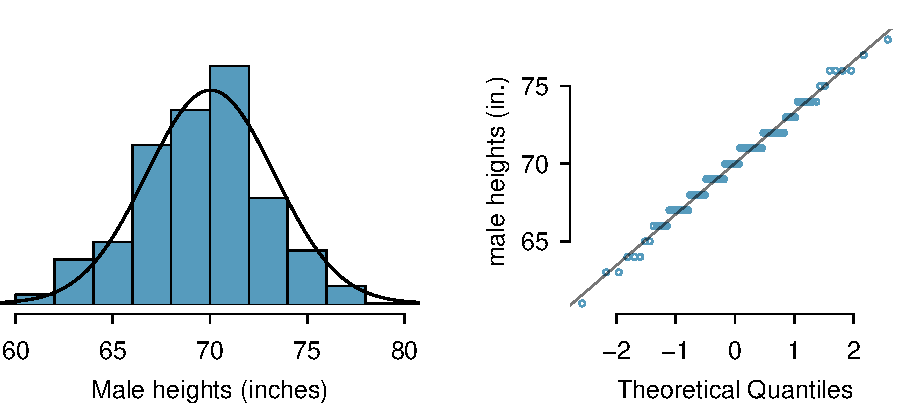
\includegraphics[width=0.8\textwidth]{03/figures/fcidMHeights/fcidMHeights}
\caption{A sample of 100 male heights. The observations are rounded to the nearest whole inch, explaining why the points appear to jump in increments in the normal probability plot.}
\label{fcidMHeights}
\end{figure}

\begin{example}{Three data sets of 40, 100, and 400 samples were simulated from a normal distribution, and the histograms and normal probability plots of the data sets are shown in Figure~\ref{normalExamples}. These will provide a benchmark for what to look for in plots of real data.} \label{normalExamplesExample}

\begin{figure}
\centering
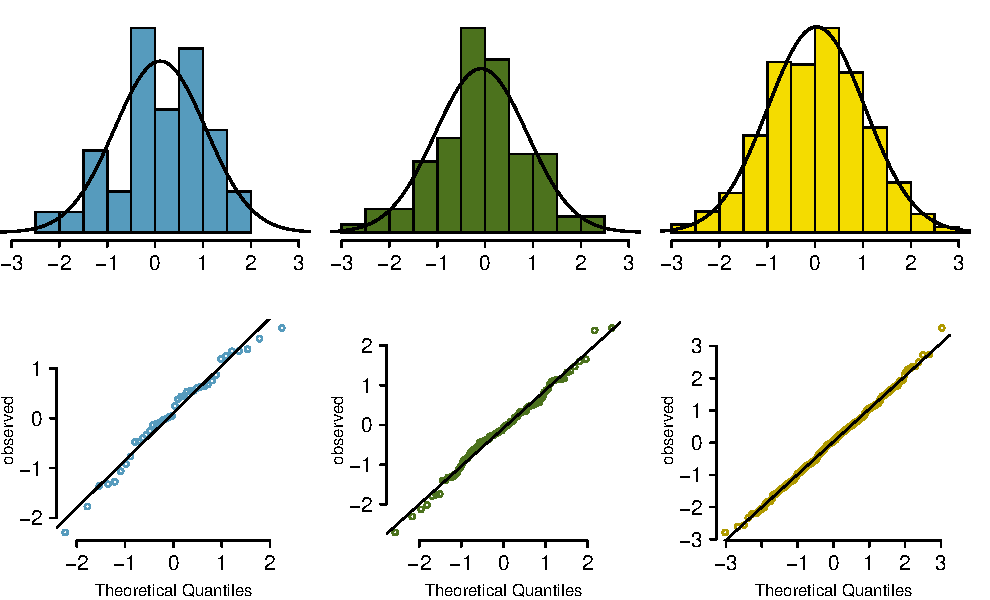
\includegraphics[width=\textwidth]{03/figures/normalExamples/normalExamples}
\caption{Histograms and normal probability plots for three simulated normal data sets; $n=40$ (left), $n=100$ (middle), $n=400$ (right).}
\label{normalExamples}
\end{figure}

The left panels show the histogram (top) and normal probability plot (bottom) for the simulated data set with 40 observations. The data set is too small to really see clear structure in the histogram. The normal probability plot also reflects this, where there are some deviations from the line. However, these deviations are not strong.

The middle panels show diagnostic plots for the data set with 100 simulated observations. The histogram shows more normality and the normal probability plot shows a better fit. While there is one observation that deviates noticeably from the line, it is not particularly extreme.

The data set with 400 observations has a histogram that greatly resembles the normal distribution, while the normal probability plot is nearly a perfect straight line. Again in the normal probability plot there is one observation (the largest) that deviates slightly from the line. If that observation had deviated 3 times further from the line, it would be of much greater concern in a real data set. Apparent outliers can occur in normally distributed data but they are rare.

Notice the histograms look more normal as the sample size increases, and the normal probability plot becomes straighter and more stable.
\end{example}

\begin{example}{Are NBA player heights normally distributed? Consider all 435 NBA players from the 2008-9 season presented in Figure~\ref{nbaNormal}.\footnote{These data were collected from \urlwofont{http://www.nba.com}.}}
We first create a histogram and normal probability plot of the NBA player heights. The histogram in the left panel is slightly left skewed, which contrasts with the symmetric normal distribution. The points in the normal probability plot do not appear to closely follow a straight line but show what appears to be a ``wave''. We can compare these characteristics to the sample of 400 normally distributed observations in Example~\ref{normalExamplesExample} and see that they represent much stronger deviations from the normal model. NBA player heights do not appear to come from a normal distribution.
\end{example}

\begin{figure}
\centering
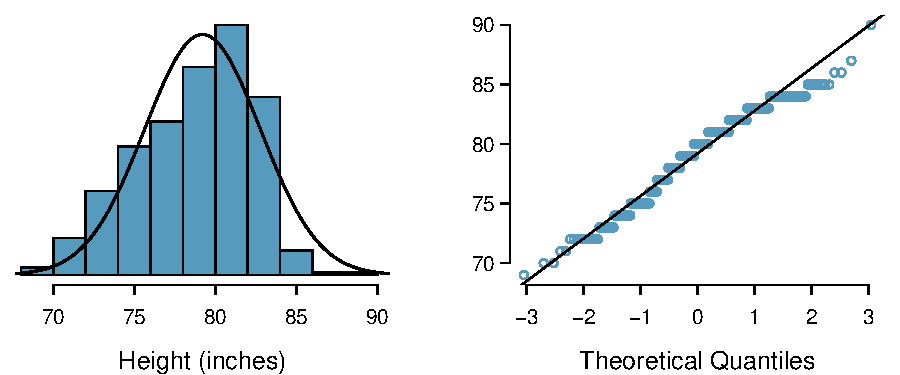
\includegraphics[width=\textwidth]{03/figures/nbaNormal/nbaNormal}
\caption{Histogram and normal probability plot for the NBA heights from the 2008-9 season.}
\label{nbaNormal}
\end{figure}

\textB{\pagebreak}

\begin{example}{Can we approximate poker winnings by a normal distribution? We consider the poker winnings of an individual over 50 days. A histogram and normal probability plot of these data are shown in Figure~\ref{pokerNormal}.}
The data are very strongly right skewed\index{skew!example: very strong} in the histogram, which corresponds to the very strong deviations on the upper right component of the normal probability plot. If we compare these results to the sample of 40 normal observations in Example~\ref{normalExamplesExample}, it is apparent that these data show very strong deviations from the normal model.
\end{example}

\begin{figure}
\centering
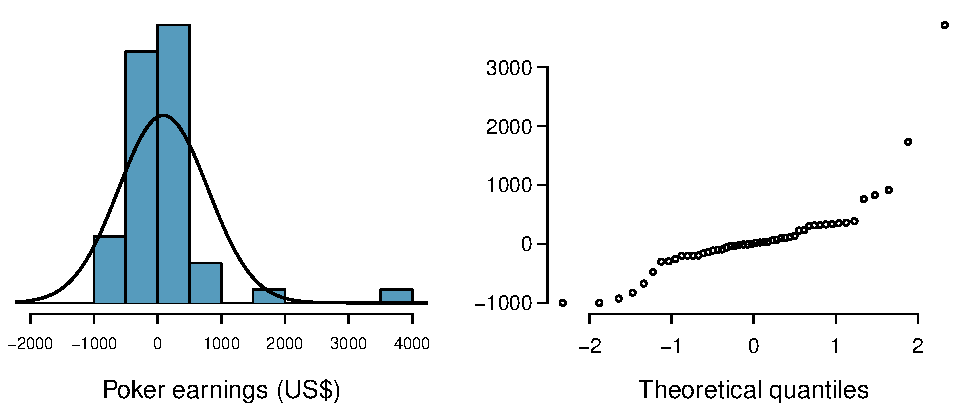
\includegraphics[width=\textwidth]{03/figures/pokerNormal/pokerNormal}
\caption{A histogram of poker data with the best fitting normal plot and a normal probability plot.}
\label{pokerNormal}
\end{figure}

\textB{\pagebreak}

\begin{exercise}\label{normalQuantileExercise}
Determine which data sets represented in Figure~\ref{normalQuantileExer} plausibly come from a nearly normal distribution. Are you confident in all of your conclusions? There are 100 (top left), 50 (top right), 500 (bottom left), and 15 points (bottom right) in the four plots.\footnote{Answers may vary a little. The top-left plot shows some deviations in the smallest values in the data set; specifically, the left tail of the data set has some outliers we should be wary of. The top-right and bottom-left plots do not show any obvious or extreme deviations from the lines for their respective sample sizes, so a normal model would be reasonable for these data sets. The bottom-right plot has a consistent curvature that suggests it is not from the normal distribution. If we examine just the vertical coordinates of these observations, we see that there is a lot of data between -20 and 0, and then about five observations scattered between 0 and 70. This describes a distribution that has a strong right skew.}
\end{exercise}

\begin{figure}
\centering
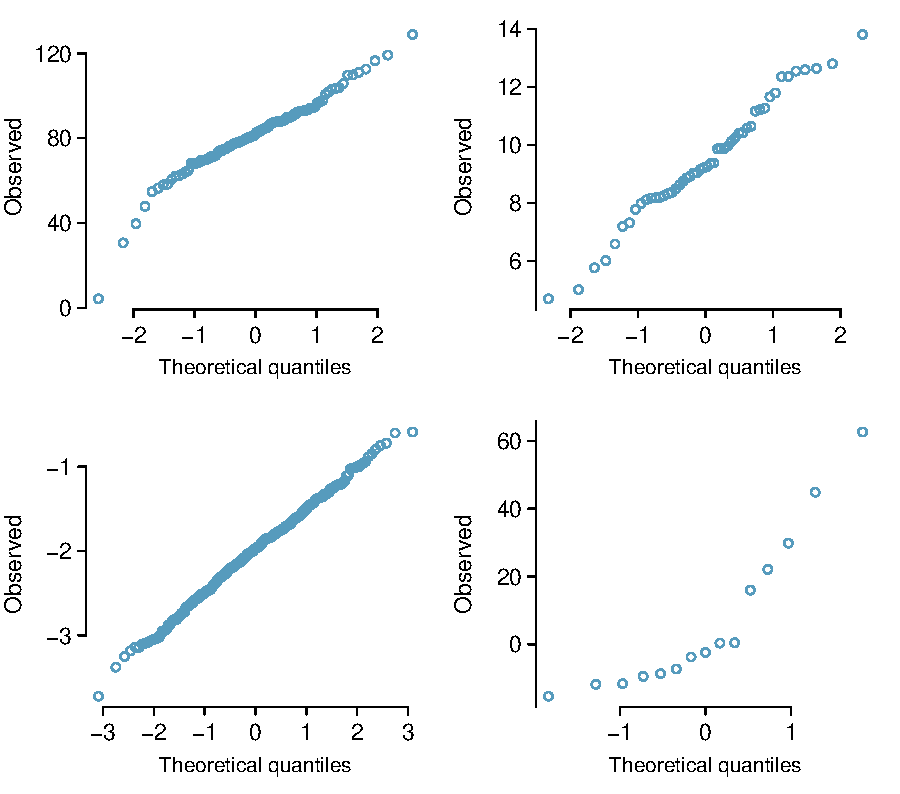
\includegraphics[width=0.9\textwidth]{03/figures/normalQuantileExer/normalQuantileExer}
\caption{Four normal probability plots for Guided Practice~\ref{normalQuantileExercise}.}
\label{normalQuantileExer}
\end{figure}

\begin{exercise} \label{normalQuantileExerciseAdditional}
Figure~\ref{normalQuantileExerAdditional} shows normal probability plots for two distributions that are skewed. One distribution is skewed to the low end (left skewed) and the other to the high end (right skewed). Which is which?\footnote{Examine where the points fall along the vertical axis. In the first plot, most points are near the low end with fewer observations scattered along the high end; this describes a distribution that is skewed to the high end. The second plot shows the opposite features, and this distribution is skewed to the low end.}
\end{exercise}

\begin{figure}
\centering
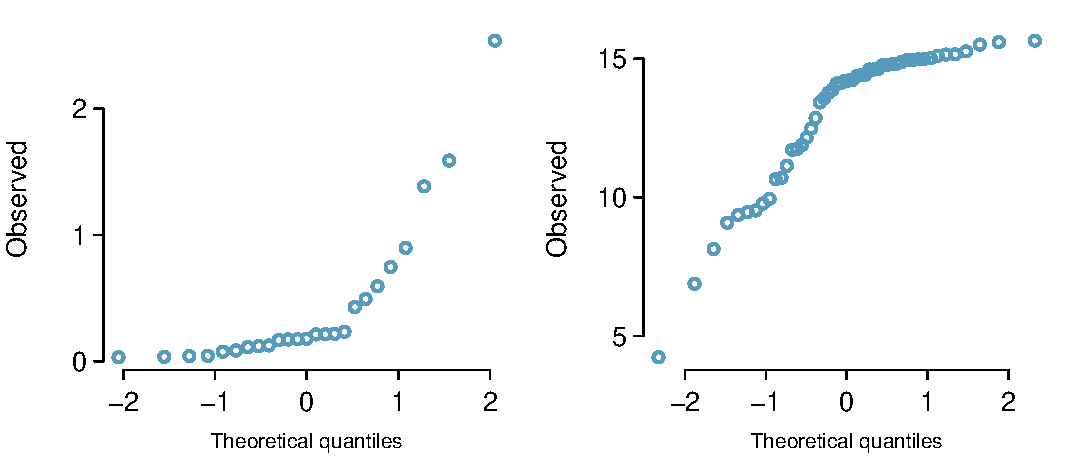
\includegraphics[width=0.9\textwidth]{03/figures/normalQuantileExer/normalQuantileExerAdditional}
\caption{Normal probability plots for Guided Practice~\ref{normalQuantileExerciseAdditional}.}
\label{normalQuantileExerAdditional}
\end{figure}

\textB{\pagebreak}

\Comment{deleted ``Constructing a normal probability plot}

%_________________
\section{Geometric distribution (special topic)}
\label{geomDist}

How long should we expect to flip a coin until it turns up \resp{heads}? Or how many times should we expect to roll a die until we get a \resp{1}? These questions can be answered using the geometric distribution. We first formalize each trial -- such as a single coin flip or die toss -- using the Bernoulli distribution, and then we combine these with our tools from probability (Chapter~\ref{probability}) to construct the geometric distribution.

\subsection{Bernoulli distribution}
\label{bernoulli}

\index{distribution!Bernoulli|(}

Stanley Milgram\index{Milgram, Stanley} began a series of experiments in 1963 to estimate what proportion of people would willingly obey an authority and give severe shocks to a stranger. Milgram found that about 65\% of people would obey the authority and give such shocks. Over the years, additional research suggested this number is approximately consistent across communities and time.\footnote{Find further information on Milgram's experiment at \par \ \ \hspace{0.2mm}\ \href{http://www.cnr.berkeley.edu/ucce50/ag-labor/7article/article35.htm}{www.cnr.berkeley.edu/ucce50/ag-labor/7article/article35.htm}.}

Each person in Milgram's experiment can be thought of as a \term{trial}. We label a person a \term{success} if she refuses to administer the worst shock. A person is labeled a \term{failure} if she administers the worst shock. Because only 35\% of individuals refused to administer the most severe shock, we denote the \term{probability of a success} with $p=0.35$. The probability of a failure is sometimes denoted with $q=1-p$.

Thus, \resp{success} or \resp{failure} is recorded for each person in the study. When an individual trial only has two possible outcomes, it is called a \termsub{Bernoulli random variable}{distribution!Bernoulli}.

\begin{termBox}{\tBoxTitle{Bernoulli random variable, descriptive}
A Bernoulli random variable has exactly two possible outcomes. We typically label one of these outcomes a ``success'' and the other outcome a ``failure''. We may also denote a success by \resp{1} and a failure by \resp{0}.}
\end{termBox}

\begin{tipBox}{\tipBoxTitle{``success'' need not be something positive}
We chose to label a person who refuses to administer the worst shock a ``success'' and all others as ``failures''. However, we could just as easily have reversed these labels. The mathematical framework we will build does not depend on which outcome is labeled a success and which a failure, as long as we are consistent.}
\end{tipBox}

Bernoulli random variables are often denoted as \resp{1} for a success and \resp{0} for a failure. In addition to being convenient in entering data, it is also mathematically handy. Suppose we observe ten trials:
\begin{center}
\resp{0} \resp{1} \resp{1} \resp{1} \resp{1} \resp{0} \resp{1} \resp{1} \resp{0} \resp{0}
\end{center}
Then the \term{sample proportion}, $\hat{p}$, is the sample mean of these observations:
\begin{eqnarray*}
\hat{p} = \frac{\text{\# of successes}}{\text{\# of trials}} = \frac{0+1+1+1+1+0+1+1+0+0}{10} = 0.6
\end{eqnarray*}%
\textB{\newpage}%
This mathematical inquiry of Bernoulli random variables can be extended even further. Because \resp{0} and \resp{1} are numerical outcomes, we can define the {mean} and {standard deviation} of a Bernoulli random variable.\footnote{If ${p}$ is the true probability of a success, then the mean of a Bernoulli random variable $X$ is given by
\begin{align*}
\mu = E[X] &= P(X=0)\times0 + P(X=1)\times1 \\
	&= (1-p)\times0 + p\times 1 = 0+p = p
\end{align*}
Similarly, the variance of $X$ can be computed:
\begin{align*}
\sigma^2 &= {P(X=0)(0-p)^2 + P(X=1)(1-p)^2} \\
	&= {(1-p)p^2 + p(1-p)^2} = {p(1-p)}
\end{align*}
The standard deviation is $\sigma=\sqrt{p(1-p)}$.}

\begin{termBox}{\tBoxTitle{Bernoulli random variable, mathematical}
If $X$ is a random variable that takes value 1 with probability of success $p$ and 0 with probability $1-p$, then $X$ is a Bernoulli random variable with mean and standard deviation
\begin{align*}
\mu &= p
	&\sigma&= \sqrt{p(1-p)}
\end{align*}}
\end{termBox}

In general, it is useful to think about a Bernoulli random variable as a random process with only two outcomes: a success or failure. Then we build our mathematical framework using the numerical labels \resp{1} and \resp{0} for successes and failures, respectively.

\index{distribution!Bernoulli|)}

\subsection{Geometric distribution}

\index{distribution!geometric|(}

\begin{example}{Dr. Smith wants to repeat Milgram's experiments but she only wants to sample people until she finds someone who will not inflict the worst shock.\footnote{This is hypothetical since, in reality, this sort of study probably would not be permitted any longer under current ethical standards.} If the probability a person will \emph{not} give the most severe shock is still 0.35 and the subjects are independent, what are the chances that she will stop the study after the first person? The second person? The third? What about if it takes her $n-1$ individuals who will administer the worst shock before finding her first success, i.e. the first success is on the $n^{th}$ person? (If the first success is the fifth person, then we say $n=5$.)} \label{waitForShocker}
The probability of stopping after the first person is just the chance the first person will not administer the worst shock: $1-0.65=0.35$. The probability it will be the second person is
\begin{eqnarray*}
&&P(\text{second person is the first to not administer the worst shock}) \\
&&\quad = P(\text{the first will, the second won't}) = (0.65)(0.35) = 0.228
\end{eqnarray*}
Likewise, the probability it will be the third person is $(0.65)(0.65)(0.35) = 0.148$.

If the first success is on the $n^{th}$ person, then there are $n-1$ failures and finally 1 success, which corresponds to the probability $(0.65)^{n-1}(0.35)$. This is the same as $(1-0.35)^{n-1}(0.35)$.
\end{example}

Example~\ref{waitForShocker} illustrates what is called the geometric distribution, which describes the waiting time until a success for \term{independent and identically distributed (iid)} Bernoulli random variables. In this case, the \emph{independence} aspect just means the individuals in the example don't affect each other, and \emph{identical} means they each have the same probability of success.

The geometric distribution from Example~\ref{waitForShocker} is shown in Figure~\ref{geometricDist35}. In general, the probabilities for a geometric distribution decrease \term{exponentially} fast.

\begin{figure}
\centering
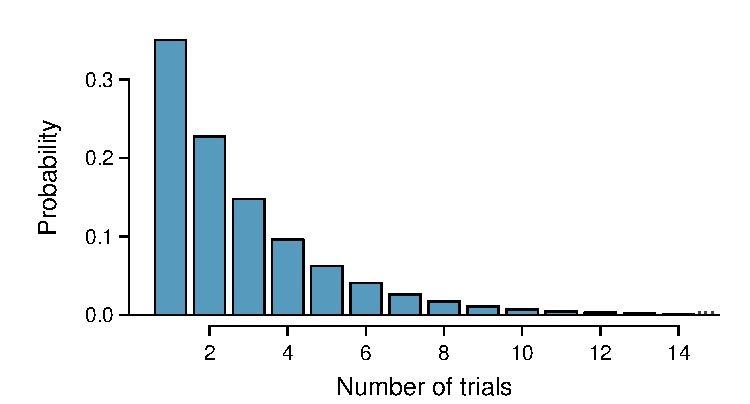
\includegraphics[width=0.8\textwidth]{03/figures/geometricDist35/geometricDist35}
\caption{The geometric distribution when the probability of success is $p=0.35$.}
\label{geometricDist35}
\end{figure}

While this text will not derive the formulas for the mean (expected) number of trials needed to find the first success or the standard deviation or variance of this distribution, we present general formulas for each.

\begin{termBox}{\tBoxTitle{Geometric Distribution\index{distribution!geometric|textbf}}
If the probability of a success in one trial is $p$ and the probability of a failure is $1-p$, then the probability of finding the first success in the $n^{th}$ trial is given by\vspace{-1.5mm}
\begin{eqnarray}
(1-p)^{n-1}p
\end{eqnarray}
The mean (i.e. expected value), variance, and standard deviation of this wait time are given by\vspace{-2.5mm}
\begin{align}
\mu &= \frac{1}{p}
	&\sigma^2&=\frac{1-p}{p^2}
	&\sigma &= \sqrt{\frac{1-p}{p^2}}
\label{geomFormulas}
\end{align}}
\end{termBox}

It is no accident that we use the symbol $\mu$ for both the mean and expected value. The mean and the expected value are one and the same.

The left side of Equation~(\ref{geomFormulas}) says that, on average, it takes $1/p$ trials to get a success. This mathematical result is consistent with what we would expect intuitively. If the probability of a success is high (e.g. 0.8), then we don't usually wait very long for a success: $1/0.8 = 1.25$ trials on average. If the probability of a success is low (e.g. 0.1), then we would expect to view many trials before we see a success: $1/0.1 = 10$ trials.

\textB{\pagebreak}

\begin{exercise}
The probability that an individual would refuse to administer the worst shock is said to be about 0.35. If we were to examine individuals until we found one that did not administer the shock, how many people should we expect to check? The first expression in Equation~(\ref{geomFormulas}) may be useful.\footnote{We would expect to see about $1/0.35 = 2.86$ individuals to find the first success.}
\end{exercise}

\begin{example}{What is the chance that Dr. Smith will find the first success within the first 4 people?} \label{marglimFirstSuccessIn4}
This is the chance it is the first ($n=1$), second ($n=2$), third ($n=3$), or fourth ($n=4$) person as the first success, which are four disjoint outcomes. Because the individuals in the sample are randomly sampled from a large population, they are independent. We compute the probability of each case and add the separate results:
\begin{eqnarray*}
&&P(n=1, 2, 3,\text{ or }4) \\
	&& \quad = P(n=1)+P(n=2)+P(n=3)+P(n=4) \\
	&& \quad = (0.65)^{1-1}(0.35) + (0.65)^{2-1}(0.35) + (0.65)^{3-1}(0.35) + (0.65)^{4-1}(0.35) \\
	&& \quad = 0.82
\end{eqnarray*}
There is an 82\% chance that she will end the study within 4~people.
\end{example}

\begin{exercise}
Determine a more clever way to solve Example~\ref{marglimFirstSuccessIn4}. Show that you get the same result.\footnote{First find the probability of the complement: $P($no success in first 4~trials$) = 0.65^4 = 0.18$. Next, compute one minus this probability: $1-P($no success in 4 trials$) = 1-0.18 = 0.82$.}
\end{exercise}

\begin{example}{Suppose in one region it was found that the proportion of people who would administer the worst shock was ``only'' 55\%. If people were randomly selected from this region, what is the expected number of people who must be checked before one was found that would be deemed a success? What is the standard deviation of this waiting time?} \label{onlyShocking55PercOfTheTimeExample}
A success is when someone will \textbf{not} inflict the worst shock, which has probability $p=1-0.55=0.45$ for this region. The expected number of people to be checked is $1/p = 1/0.45 = 2.22$ and the standard deviation is $\sqrt{(1-p)/p^2} = 1.65$.
\end{example}

\begin{exercise}
Using the results from Example~\ref{onlyShocking55PercOfTheTimeExample}, $\mu = 2.22$ and $\sigma = 1.65$, would it be appropriate to use the normal model to find what proportion of experiments would end in 3 or fewer trials?\footnote{No. The geometric distribution is always right skewed and can never be well-approximated by the normal model.}
\end{exercise}

The independence assumption is crucial to the geometric distribution's accurate description of a scenario. Mathematically, we can see that to construct the probability of the success on the $n^{th}$ trial, we had to use the Multiplication Rule for Independent Processes. It is no simple task to generalize the geometric model for dependent trials.

%\begin{exercise}
%The independence assumption is crucial to the geometric distribution's accurate description of a scenario. Why?\footnote{Independence simplified the situation. Mathematically, we can see that to construct the probability of the success on the $n^{th}$ trial, we had to use the Multiplication Rule for Independent processes. It is no simple task to generalize the geometric model for dependent trials.}
%\end{exercise}
\index{distribution!geometric|)}


\textB{\pagebreak}

\section{Binomial distribution}
\label{binomialModel}

\index{distribution!binomial|(}

\begin{example}{Suppose we randomly selected four individuals to participate in the ``shock" study. What is the chance exactly one of them will be a success?  Let's call the four people Allen ($A$), Brittany ($B$), Caroline ($C$), and Damian ($D$) for convenience. Also, suppose 35\% of people are successes as in the previous version of this example.}\label{oneRefuser}
Let's consider a scenario where one person refuses:
\begin{eqnarray*}
&&P(A=\text{\resp{refuse}},\text{ }B=\text{\resp{shock}},\text{ }C=\text{\resp{shock}},\text{ }D=\text{\resp{shock}}) \\
 &&\quad =  P(A=\text{\resp{refuse}})\ P(B=\text{\resp{shock}})\ P(C=\text{\resp{shock}})\ P(D=\text{\resp{shock}}) \\
 &&\quad =  (0.35)  (0.65)  (0.65)  (0.65) = (0.35)^1 (0.65)^3 = 0.096
\end{eqnarray*}
But there are three other scenarios: Brittany, Caroline, or Damian could have been the one to refuse. In each of these cases, the probability is again $(0.35)^1(0.65)^3$. These four scenarios exhaust all the possible ways that exactly one of these four people could refuse to administer the most severe shock, so the total probability is $4\times(0.35)^1(0.65)^3 = 0.38$.
\end{example}

\begin{exercise}
Verify that the scenario where Brittany is the only one to refuse to give the most severe shock has probability $(0.35)^1(0.65)^3$.\footnote{$P(A=\text{\resp{shock}},\text{ }B=\text{\resp{refuse}},\text{ }C=\text{\resp{shock}},\text{ }D=\text{\resp{shock}}) = (0.65)(0.35)(0.65)(0.65) = (0.35)^1(0.65)^3$.}
\end{exercise}

\Comment{rename section ``binomial formula and add section on binomial distribution.}
%\subsection{The binomial distribution}
\subsection{Binomial formula}
\Cut{The scenario outlined in Example~\ref{oneRefuser} is a special case of what is called the binomial distribution. The \termsub{binomial distribution}{distribution!binomial} describes the probability of having exactly $k$ successes in $n$ independent Bernoulli trials with probability of a success $p$}\Add{To solve the scenario outlined in Example~\ref{oneRefuser} we use what is called the \term{Binomal Formula}.  The binomal formula gives the probability of having $k$ successes in $n$ independent rials with probability of a success $p$.} (in Example~\ref{oneRefuser}, $n=4$, $k=1$, $p=0.35$). \Cut{We would like to determine the probabilities associated with the binomial distribution more generally, i.e. we want a formula where we can use $n$, $k$, and $p$ to obtain the probability. To do this, we reexamine each part of the example.}\Add{In order to develop this formula, we reexamine each part of the example.}

There were four individuals who could have been the one to refuse, and each of these four scenarios had the same probability. Thus, we could identify the final probability as
\begin{eqnarray}
[\text{\# of scenarios}] \times P(\text{single scenario})
\label{genBinomialFormula}
\end{eqnarray}
The first component of this equation is the number of ways to arrange the $k=1$ successes among the $n=4$ trials. The second component is the probability of any of the four (equally probable) scenarios.

Consider $P($single scenario$)$ under the general case of $k$ successes and $n-k$ failures in the $n$ trials. In any such scenario, we apply the Multiplication Rule for independent events:
\begin{eqnarray*}
p^k(1-p)^{n-k}
\end{eqnarray*}
This is our general formula for $P($single scenario$)$.

\textB{\pagebreak}

Secondly, we introduce a general formula for the number of ways to choose $k$ successes in $n$ trials, i.e. arrange $k$ successes and $n-k$ failures:
\begin{eqnarray*}
{n\choose k} = \frac{n!}{k!(n-k)!}
\end{eqnarray*}
The quantity ${n\choose k}$ is read \term{n choose k}.\footnote{Other notation for $n$ choose $k$ includes $_nC_k$, $C_n^k$, and $C(n,k)$.} The exclamation point notation (e.g. $k!$) denotes a \term{factorial}\label{factorialDefinitionInTheBinomialSection} expression.
\begin{eqnarray*}
&& 0! = 1 \label{zeroFactorial} \\
&& 1! = 1 \\
&& 2! = 2\times1 = 2 \\
&& 3! = 3\times2\times1 = 6 \\
&& 4! = 4\times3\times2\times1 = 24 \\
&& \vdots \\
&& n! = n\times(n-1)\times...\times3\times2\times1
\end{eqnarray*}
Using the formula, we can compute the number of ways to choose $k=1$ successes in $n=4$ trials:
\begin{eqnarray*}
{4 \choose 1} = \frac{4!}{1!(4-1)!} =  \frac{4!}{1!3!} 
	= \frac{4\times3\times2\times1}{(1)(3\times2\times1)} = 4
\end{eqnarray*}
This result is exactly what we found by carefully thinking of each possible scenario in Example~\ref{oneRefuser}.

Substituting $n$ choose $k$ for the number of scenarios and $p^k(1-p)^{n-k}$ for the single scenario probability in Equation~(\ref{genBinomialFormula}) yields the general binomial formula.

\Comment{changed ``binomial distribution" to ``binomial formula" and deleted mean, sd, and variance from termbox}

\begin{termBox}{\tBoxTitle{Binomial formula} Suppose the probability of a single trial being a success is $p$. Then the probability of observing exactly $k$ successes in $n$ independent trials is given by\vspace{-1mm}
\begin{eqnarray}
{n\choose k}p^k(1-p)^{n-k} = \frac{n!}{k!(n-k)!}p^k(1-p)^{n-k}
\label{binomialFormula}
\end{eqnarray}
}
\end{termBox}

\begin{tipBox}{\tipBoxTitle{Is it binomial? Four conditions to check.\label{isItBinomialTipBox}}
(1) The trials are independent. \\
(2) The number of trials, $n$, is fixed. \\
(3) Each trial outcome can be classified as a \emph{success} or \emph{failure}. \\
(4) The probability of a success, $p$, is the same for each trial.}
\end{tipBox}

\textB{\pagebreak}

\begin{example}{What is the probability that 3 of 8 randomly selected students will refuse to administer the worst shock, i.e. 5 of 8 will?}
We would like to apply the binomial model, so we check our conditions. The number of trials is fixed ($n=8$) (condition 2) and each trial outcome can be classified as a success or failure (condition 3). Because the sample is random, the trials are independent (condition~1) and the probability of a success is the same for each trial (condition~4).

In the outcome of interest, there are $k=3$ successes in $n=8$ trials, and the probability of a success is $p=0.35$. So the probability that 3 of 8 will refuse is given by
\begin{eqnarray*}
{ 8 \choose 3}(0.35)^3(1-0.35)^{8-3}
	&=& \frac{8!}{3!(8-3)!}(0.35)^3(1-0.35)^{8-3} \\
	&=& \frac{8!}{3!5!}(0.35)^3(0.65)^5
\end{eqnarray*}
Dealing with the factorial part:
\begin{eqnarray*}
\frac{8!}{3!5!} = \frac{8\times7\times6\times5\times4\times3\times2\times1}{(3\times2\times1)(5\times4\times3\times2\times1)} = \frac{8\times7\times6}{3\times2\times1} = 56
\end{eqnarray*}
Using $(0.35)^3(0.65)^5 \approx 0.005$, the final probability is about $56*0.005 = 0.28$.
\end{example}

\begin{tipBox}{\tipBoxTitle{computing binomial probabilities}
The first step in using the binomial model is to check that the model is appropriate. The second step is to identify $n$, $p$, and $k$. The final step is to apply the formulas and interpret the results.}
\end{tipBox}

\begin{tipBox}{\tipBoxTitle{computing $n$ choose $k$ \color{red} CUT THIS BOX}
In general, it is useful to do some cancelation in the factorials immediately. Alternatively, many computer programs and calculators have built in functions to compute $n$ choose $k$, factorials, and even entire binomial probabilities.}
\end{tipBox}

\Comment{moved this exercise to next subsection}
\Cut{
\begin{exercise}
If you ran a study and randomly sampled 40 students, how many would you expect to refuse to administer the worst shock? What is the standard deviation of the number of people who would refuse? Equation~(\ref{binomialStats}) may be useful.\footnote{We are asked to determine the expected number (the mean) and the standard deviation, both of which can be directly computed from the formulas in Equation~(\ref{binomialStats}): $\mu=np = 40\times 0.35 = 14$ and $\sigma = \sqrt{np(1-p)} = \sqrt{40\times 0.35\times 0.65} = 3.02$. Because very roughly 95\% of observations fall within 2 standard deviations of the mean (see Section~\ref{variability}), we would probably observe at least 8 but less than 20 individuals in our sample who would refuse to administer the shock.}
\end{exercise}
}

\begin{exercise}
The probability that a random smoker will develop a severe lung condition in his or her lifetime is about $0.3$. If you have 4 friends who smoke, are the conditions for the binomial model satisfied?\footnote{One possible answer: if the friends know each other, then the independence assumption is probably not satisfied. For example, acquaintances may have similar smoking habits.}
\end{exercise}

\begin{exercise}
\label{noMoreThanOneFriendWSevereLungCondition}%
Suppose these four friends do not know each other and we can treat them as if they were a random sample from the population. Is the binomial model appropriate? What is the probability that (a) none of them will develop a severe lung condition? (b) One will develop a severe lung condition? (c) That no more than one will develop a severe lung condition?\footnote{To check if the binomial model is appropriate, we must verify the conditions. (i) Since we are supposing we can treat the friends as a random sample, they are independent. (ii) We have a fixed number of trials ($n=4$). (iii) Each outcome is a success or failure. (iv) The probability of a success is the same for each trials since the individuals are like a random sample ($p=0.3$ if we say a ``success'' is someone getting a lung condition, a morbid choice). Compute parts (a) and (b) from the binomial formula in Equation~\eqref{binomialFormula}: $P(0) =  {4 \choose 0} (0.3)^0 (0.7)^4 = 1\times1\times0.7^4 = 0.2401$, $P(1) = {4 \choose 1} (0.3)^1(0.7)^{3} = 0.4116$. Note: $0!=1$, as shown on page~\pageref{zeroFactorial}. Part (c) can be computed as the sum of parts (a) and (b): $P(0) + P(1) = 0.2401 + 0.4116 = 0.6517$. That is, there is about a 65\% chance that no more than one of your four smoking friends will develop a severe lung condition.}
\end{exercise}

\begin{exercise}
What is the probability that at least 2 of your 4 smoking friends will develop a severe lung condition in their lifetimes?\footnote{The complement (no more than one will develop a severe lung condition) as computed in Guided Practice~\ref{noMoreThanOneFriendWSevereLungCondition} as 0.6517, so we compute one minus this value: 0.3483.}
\end{exercise}

\begin{exercise}
Suppose you have 7 friends who are smokers and they can be treated as a random sample of smokers. \Cut{(a) How many would you expect to develop a severe lung condition, i.e. what is the mean? (b)}What is the probability that at most 2 of your 7 friends will develop a severe lung condition.\footnote{$P($0, 1, or 2 develop severe lung condition$) = P(k=0) + P(k=1)+P(k=2) = 0.6471$.}
\end{exercise}

Below we consider the first term in the binomial probability, $n$ choose $k$ under some special scenarios.

\begin{exercise}
Why is it true that ${n \choose 0}=1$ and ${n \choose n}=1$ for any number $n$?\footnote{Frame these expressions into words. How many different ways are there to arrange 0 successes and $n$ failures in $n$ trials? (1 way.) How many different ways are there to arrange $n$ successes and 0 failures in $n$ trials? (1 way.)}
\end{exercise}

\begin{exercise}
How many ways can you arrange one success and $n-1$ failures in $n$ trials? How many ways can you arrange $n-1$ successes and one failure in $n$ trials?\footnote{One success and $n-1$ failures: there are exactly $n$ unique places we can put the success, so there are $n$ ways to arrange one success and $n-1$ failures. A similar argument is used for the second question. Mathematically, we show these results by verifying the following two equations:
\begin{eqnarray*}
{n \choose 1} = n, \qquad {n \choose n-1} = n
\end{eqnarray*}}
\end{exercise}

\begin{example}{There are 13 marbles in a bag.  4 are blue and 9 are red.  Randomly draw 5 marbles \emph{without replacement}.  Find the probability you get exactly 3 blue marbles.}Because the probability of success $p$ is not the same for each trial, we cannot use the binomial formula.  However, we can use the same logic to arrive at the following answer.  
\begin{align*}
P(x = 3) &= (\text{\# of combinations with 3 blue})\times P(\text{3 blue and 2 red in a \emph{specific} order}) \\
&={5\choose 3}\times P(\text{RRRBB}) \\
&= {5\choose 3}(\frac{4}{13}\times \frac{3}{12}\times \frac{2}{11} \times \frac{9}{10} \times \frac{8}{9}) \\
&= 0.1112
\end{align*}
\end{example}

\Comment{added this section on calculator and binomial}

\subsection{Calculator: binomial probabilities}
\label{calculatorBinomial}

\begin{termBox}{\tBoxTitle{TI calculator: Computing the binomial coefficient: ${n\choose k}$}
Use \textbf{MATH, PRB, nCr} to evaluate $n$ choose $r$. Here r and k are different letters for the same quantity.  e.g.: 5 nCr 3 means 5 choose 3.
\begin{enumerate}
\item Type the value of n.
\item Select MATH.
\item Right arrow to PRB.
\item Choose 3:nCr.
\item Type the value of k.
\item Hit ENTER.
\end{enumerate}
}
\end{termBox}

\begin{termBox}{\tBoxTitle{TI: calculator: Computing binomial formula: $P(x = k)={n\choose k}p^k(1-p)^{n-k}$} 
Use \textbf{2ND VARS, binompdf} to evaluate the probability of \emph{exactly} $k$ occurrences out of $n$ independent trials of an event with probability $p$.  
\begin{enumerate}
\item Select 2ND VARS (i.e. DISTR)
\item Choose A:binompdf  (use the down arrow).
\item Let trials be $n$.
\item Let p be $p$
\item Let x value be $k$.
\item Select Paste and hit ENTER.
\newline
\begin{itemize}
\item[TI-83: ] Do steps 1 - 2, then enter $n$, $p$, and $k$ separated by commas as follows:  binompdf($n$, $p$, $k$).  Then hit ENTER. 
\end{itemize}
\end{enumerate}
}
\end{termBox}

\begin{termBox}{\tBoxTitle{TI calculator: Computing $P(x \le k)= {n\choose 0}p^0(1-p)^{n-0} + ... + {n\choose k}p^k(1-p)^{n-k}$} 
Use \textbf{2ND VARS, binomcdf} to evaluate the cumulative probability of \emph{at least} $k$ occurrences out of $n$ independent trials of an event with probability $p$.  
\begin{enumerate}
\item Select 2ND VARS (i.e. DISTR)
\item Choose B:binomcdf  (use the down arrow).
\item Let trials be $n$.
\item Let p be $p$
\item Let x value be $k$.
\item Select Paste and hit ENTER.
\begin{itemize}
\item[TI-83: ] Do steps 1 - 2, then enter $n$, $p$, and $k$ separated by commas as follows: binomcdf($n$, $p$, $k$).  Then hit ENTER.
\end{itemize}
\end{enumerate}
}
\end{termBox}

\begin{exercise}Find the number of ways of arranging 3 blue marbles and 2 red marbles.\footnote{Using 5 nCr 3 gives 10. }
\end{exercise}

\begin{exercise}There are 13 marbles in a bag.  4 are blue and 9 are red.  Randomly draw 5 marbles \emph{with replacement}.  Find the probability you get exactly 3 blue marbles.\footnote{using binompdf(5, 4/13, 3) gives 0.1396.}
\end{exercise}

\begin{exercise}There are 13 marbles in a bag.  4 are blue and 9 are red.  Randomly draw 5 marbles \emph{with replacement}.  Find the probability you get \emph{at least} 3 blue marbles.\footnote{using binomcdf(5, 4/13, 3) gives 0.9662.}
\end{exercise}

\subsection{Binomal Distribution}
\Add{
Consider Guided Practice~\ref{noMoreThanOneFriendWSevereLungCondition}.  We asked many probability questions regarding this scenario that could be solved using the binomial formula.  Instead of looking at it piecewise, we could describe the entire \emph{distribution} of possible values and their corresponding probabilities.  Since there are 4 smoking friends, the possible outcomes of the variable ``how many of the 4 will develop a severe lung condition in their lifetime" are: 0, 1, 2, 3, 4.  We can make a distribution table as we did previously.  Recall that the probability that a random smoker will develop a severe lung condition in his or her lifetime is about $0.3$.
}
\Comment{TODO(David) add histogram}

\begin{table}[hr]
\centering
\begin{tabular}{l l}
$x_i$ & $p_i$ \\
\hline
0 &  ${4\choose 0}(0.3)^0(0.7)^{4} = 0.058$ \vspace{1mm}\\
1 &  ${4\choose 1}(0.3)^1(0.7)^{3} = 0.268$  \vspace{1mm}\\
2 & ${4\choose 2}(0.3)^2(0.7)^{2} = 0.242$  \vspace{1mm}\\
3 & ${4\choose 3}(0.3)^3(0.7)^{1} = 0.075$  \vspace{1mm}\\
4 & ${4\choose 4}(0.3)^4(0.7)^{0} = 0.008$  \vspace{1mm}
\end{tabular}
\caption{Probability Distribution of ``How many of 4 smoking friends will develop a severe lung condition in their lifetime".  This distribution is a binomial distribution.  To rounding error, these probabilities add up to 1. }
\label{binomDistrSmokers}
\end{table}

\Add{
Since this is a probability distribution we could find the mean and standard deviation of it using the formulas from the previous chapter.  Those formulas require a lot of calculations, so it is fortunate that there are shortcut formulas for the mean and the standard deviation of a binomial random variable.
}

\begin{termBox}{\tBoxTitle{Mean and standard deviation of the binomial distribution}
For a binomial distribution with parameters $n$ and $p$, where $n$ is the number of trials and $p$ is the probability of a success, the mean and standard deviation of the number of observed successes are\vspace{-2mm}
\begin{align}
\mu_x &= np
	&\sigma_x &= \sqrt{np(1-p)}
\label{binomialStats}
\end{align}
}
\end{termBox}

\Add{
\begin{example}{If the probability that a random smoker will develop a severe lung condition in his or her lifetime is $0.3$ and you have 40 smoking friends, how many would you expect to develop such a condition? What is the standard deviation of the number of people who would develop such a condition? Equation~(\ref{binomialStats}) may be useful.}We are asked to determine the expected number (the mean) and the standard deviation, both of which can be directly computed from the formulas in Equation~(\ref{binomialStats}):
 \begin{align*}
\mu&=np = 40\times 0.3 = 12 \\
 \sigma &= \sqrt{np(1-p)} = \sqrt{40\times 0.3\times 0.7} = 2.9
\end{align*}
Because very roughly 95\% of observations fall within 2 standard deviations of the mean (see Section~\ref{variability}), we would probably observe at least 6 but less than 28 individuals in our sample who develop a severe lung condition in their lifetimes.
\end{example}

\Comment{ref graph}
Look again at the graph ~\ref{} and note that the mean and standard deviation calculated match up with graph.  This graph is right-skewed. 

\begin{exercise}Describe the graph of the binomial distribution if $p$ had been 0.5.  Let $n$ remain 4. \footnote{It would be symmetric.  The mean would be $40\times 0.5 = 20$ and the standard deviation would be $ \sqrt{40\times 0.5\times 0.5} = 3.16$.}
\end{exercise}

\begin{exercise}Describe the graph of the binomial distribution if $p$ had been 0.7.  Let $n$ remain 4.?\footnote{The mean would be $40\times 0.7 = 28$ and the standard deviation would be $ \sqrt{40\times 0.7\times 0.3} = 2.9$.  The graph would be left-skewed.  In fact, is is the same as the graph with $n=4$ and $p=0.3$ but flipped horizontally.}
\end{exercise}

It is useful to consider what happens to the binomial distribution as $n$ and $p$ change.  It is intuitive that when $p=0.5$, as $n$ increases, the distribution becomes more normal.  It is less intuitive but nevertheless true that for any value of $p$, no matter how extreme (meaning how close to 0 or 1), as $n$ increases, the distribution will become more normal.\footnote{These websites have excellent interactive applets that let you see how the binomial distribution changes as you change $n$ and $p$.  
\urlwofont{http://bcs.whfreeman.com/ips4e/cat_010/applets/CLT-Binomial.html}

\urlwofont{http://www.stat.berkeley.edu/~stark/Java/Html/BinHist.htm}}
The next section will introduce a rule of thumb for when the binomial distribution can be well approximated by a normal distribution.
}

\subsection{Normal approximation to the binomial distribution}

\index{distribution!binomial!normal approximation|(}

\Comment{ changed k=59 to 60 to make phat be a rounder number in last section}
The binomial formula is cumbersome when the sample size ($n$) is large, particularly when we consider a range of observations. In some cases we may use the normal distribution as an easier and faster way to estimate binomial probabilities.

\begin{example}{Approximately 20\% of the US population smokes cigarettes. A local government believed their community had a lower smoker rate and commissioned a survey of 400 randomly selected individuals. The survey found that only 60 of the 400 participants smoke cigarettes. If the true proportion of smokers in the community was really 20\%, what is the probability of observing 60 or fewer smokers in a sample of 400 people?}\label{exactBinomialForN400P20SmokerExample}
We leave the usual verification that the four conditions for the binomial model are valid as an exercise.

The question posed is equivalent to asking, what is the probability of observing $k=0$, 1, ..., 59, or 60 smokers in a sample of $n=400$ when $p=0.20$? We can compute these 61 different probabilities and add them together to find the answer:
\begin{align*}
&P(k=0\text{ or }k=1\text{ or }\cdots\text{ or } k=60) \\
	&\qquad= P(k=0) + P(k=1) + \cdots + P(k=60) \\
	&\qquad=0.0061
\end{align*}
If the true proportion of smokers in the community is $p=0.20$, then the probability of observing 60 or fewer smokers in a sample of $n=400$ is less than 0.0061.
\end{example}

The computations in Example~\ref{exactBinomialForN400P20SmokerExample} are tedious and long. In general, we should avoid such work if an alternative method exists that is faster, easier, and still accurate. Recall that calculating probabilities of a range of values is much easier in the normal model. We might wonder, is it reasonable to use the normal model in place of the binomial distribution? Surprisingly, yes, if certain conditions are met.

\begin{exercise}
Here we consider the binomial model when the probability of a success is $p=0.10$. Figure~\ref{fourBinomialModelsShowingApproxToNormal} shows four hollow histograms for simulated samples from the binomial distribution using four different sample sizes: $n=10, 30, 100, 300$. What happens to the shape of the distributions as the sample size increases? What distribution does the last hollow histogram resemble?\footnote{The distribution is transformed from a blocky and skewed distribution into one that rather resembles the normal distribution in last hollow histogram}
\end{exercise}

\begin{figure}[h]
\centering
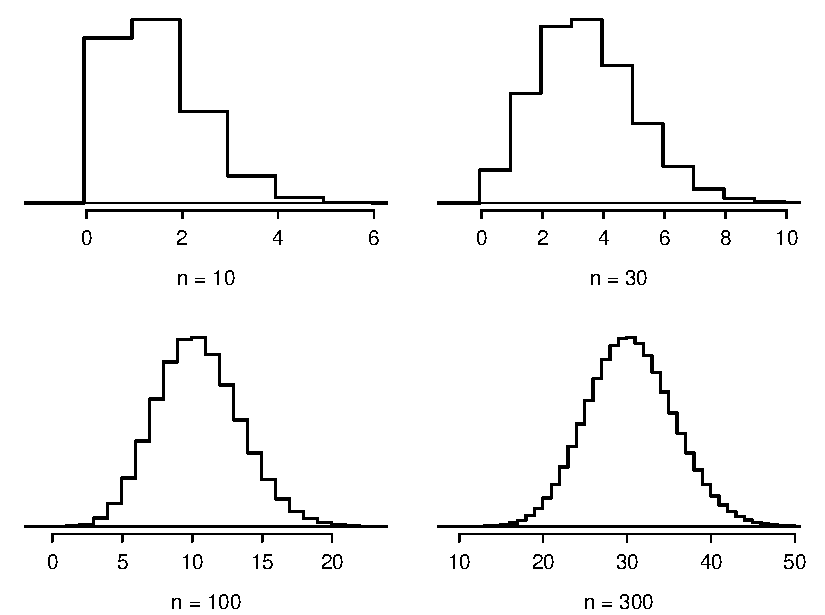
\includegraphics[width=0.9\textwidth]{03/figures/fourBinomialModelsShowingApproxToNormal/fourBinomialModelsShowingApproxToNormal}
\caption{Hollow histograms of samples from the binomial model when $p=0.10$. The sample sizes for the four plots are $n=10$, 30, 100, and 300, respectively.}
\label{fourBinomialModelsShowingApproxToNormal}
\end{figure}

\begin{termBox}{\tBoxTitle{Normal approximation of the binomial distribution}
The binomial distribution with probability of success $p$ is nearly normal when the sample size $n$ is sufficiently large that $np$ and $n(1-p)$ are both at least 10. The approximate normal distribution has parameters corresponding to the mean and standard deviation of the binomial distribution:\vspace{-1.5mm}
\begin{align*}
\mu &= np
&&\sigma= \sqrt{np(1-p)}
\end{align*}}
\end{termBox}

The normal approximation may be used when computing the range of many possible successes. For instance, we may apply the normal distribution to the setting of Example~\ref{exactBinomialForN400P20SmokerExample}.

\Cut{
\begin{example}{How can we use the normal approximation to estimate the probability of observing 59 or fewer smokers in a sample of 400, if the true proportion of smokers is $p=0.20$?} \label{approxBinomialForN400P20SmokerExample}
Showing that the binomial model is reasonable was a suggested exercise in Example~\ref{exactBinomialForN400P20SmokerExample}. We also verify that both $np$ and $n(1-p)$ are at least 10:
\begin{align*}
np&=400\times 0.20=80
&n(1-p)&=400\times 0.8=320
\end{align*}
With these conditions checked, we may use the normal approximation in place of the binomial distribution using the mean and standard deviation from the binomial model:
\begin{align*}
\mu &= np = 80
&\sigma &= \sqrt{np(1-p)} = 8
\end{align*}
We want to find the probability of observing fewer than 59 smokers using this model.
\end{example}

\begin{exercise}
Use the normal model $N(\mu=80, \sigma=8)$ to estimate the probability of observing fewer than 59 smokers. Your answer should be approximately equal to the solution of Example~\ref{exactBinomialForN400P20SmokerExample}: 0.0041.\footnote{Compute the Z score first: $Z=\frac{59 - 80}{8} = -2.63$. The corresponding left tail area is 0.0043.}
\end{exercise}
}

\Add{
\begin{example}{Use the normal approximation to estimate the probability of observing 60 or fewer smokers in a sample of 400, if the true proportion of smokers is $p=0.20$?} \label{approxBinomialForN400P20SmokerExample}
Showing that the binomial model is reasonable was a suggested exercise in Example~\ref{exactBinomialForN400P20SmokerExample}. We also verify that both $np$ and $n(1-p)$ are at least 10:
\begin{align*}
np&=400(0.20)=80\ge 10 \\
n(1-p)&=400(0.8)=320\ge 10
\end{align*}
With these conditions checked, we may use the normal approximation in place of the binomial distribution using the mean and standard deviation from the binomial model:
\begin{align*}
\mu &= np = 400(0.2)=80 \\
\sigma &= \sqrt{np(1-p)} = \sqrt{400(0.2)(0.8)}= 8
\end{align*}
We want to find the probability of observing 60 or fewer smokers using this model.  We know that this probability will be small because 60 is more than 2 standard deviations below the mean of 80.

Compute the Z score: $Z=\frac{60 - 80}{8} = -2.5$. 

Find the area in the left-hand tail: $P(Z < -2.5) = 0.0062$

This probability of 0.0062 using the normal approximation is very close to the true probability of 0.0061 using the binomial distribution.

\end{example}

\begin{exercise}
Use normal approximation, if applicable, to estimate the probability of getting greater than 15 sixes in 100 rolls of a fair die.\footnote{$np=100\times 1/6=16.7\ge 10$ and 
$n(1-p)=100\times 5/6=83.3\ge 10$  

$\mu=np=100(1/6)=16.7; \sigma=\sqrt{np(1-p)}=\sqrt{100\times (1/6)(5/6)}=3.7$ 

$Z=\frac{15 - 16.7}{3.7} = -0.46$. 

$P(Z > -0.46) = 0.677$
}
\end{exercise}
}

\textB{\pagebreak}

\Comment{made this a special topic, and added a brief statement about the continuity correction}

\subsection{The normal approximation breaks down on small intervals (special topic)}

\begin{caution}
{The normal approximation may fail on small intervals}
{The normal approximation to the binomial distribution tends to perform poorly when estimating the probability of a small range of counts, even when the conditions are met.}
\end{caution}

Suppose we wanted to compute the probability of observing 69, 70, or 71 smokers in 400 when $p=0.20$. With such a large sample, we might be tempted to apply the normal approximation and use the range 69 to 71. However, we would find that the binomial solution and the normal approximation notably differ:
\begin{align*}
\text{Binomial:}&\ 0.0703
&\text{Normal:}&\ 0.0476
\end{align*}
We can identify the cause of this discrepancy using Figure~\ref{normApproxToBinomFail}, which shows the areas representing the binomial probability (outlined) and normal approximation (shaded). Notice that the width of the area under the normal distribution is 0.5 units too slim on both sides of the interval.  \Add{This is because the binomial distribution is \emph{discrete} and the each bar is centered over an integer value.  Looking closely at Figure~\ref{normApproxToBinomFail}, we see that the bar corresponding to 69 begins at 68.5 and ends at 69.5, the bar corresponding to 70 begins at 69.5 and ends at 70.5, and the bar corresponding to 71 begins at 70.5 and ends at 71.5.}

\Comment{ added " from 68.5 to 71.5 " to caption of figure.}
\begin{figure}[h]
\centering
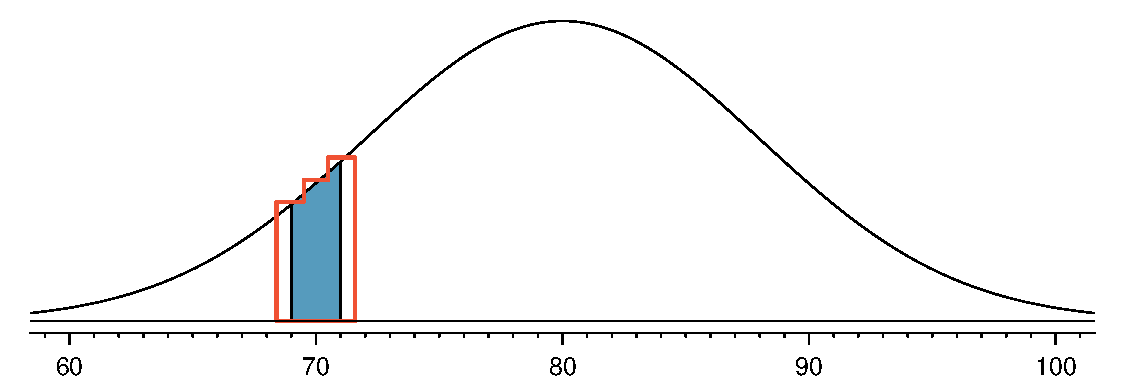
\includegraphics[width=\textwidth]{03/figures/normApproxToBinomFail/normApproxToBinomFail}
\caption{A normal curve with the area between 69 and 71 shaded. The outlined area from 68.5 to 71.5 represents the exact binomial probability.}
\label{normApproxToBinomFail}
\end{figure}

\Comment{replace first tipbox with second?}

\begin{tipBox}{\tipBoxTitle{Improving the accuracy of the normal approximation to the binomial distribution}
The normal approximation to the binomial distribution for intervals of values is usually improved if cutoff values are modified slightly. The cutoff values for the lower end of a shaded region should be reduced by 0.5, and the cutoff value for the upper end should be increased by 0.5.  }
\end{tipBox}


\begin{tipBox}{\tipBoxTitle{Improving the accuracy of the normal approximation to the binomial distribution}
The normal approximation to the binomial distribution for intervals of values is usually improved if cutoff values for the lower end of a shaded region are reduced by 0.5 and the cutoff value for the upper end are increased by 0.5.  This correction is called the continuity correction and accounts for the fact that the binomial distribution is discrete.  }
\end{tipBox}

\Add{
\begin{example}{Use the method described to find a more accurate estimate for the probability of observing 69, 70, or 71 smokers in 400 when $p=0.20$.}
Instead of standardizing 69 and 71, we will standardize 68.5 and 71.5.

$Z = \frac{68.5-80}{8}=-1.4375$

$Z = \frac{71.5-80}{8} =-1.0625$

$P(-1.4375 < Z < -1.0625) =0.0687$

Note that this probability of 0.0687 is much closer to the true value of 0.0703 than the value of 0.0476 we calculated using normal approximation without the continuinty correction.

\end{example}

}

\Cut{
a TIp to add extra area when applying the normal approximation is most often useful when examining a range of observations. While it is possible to apply it when computing a tail area, the benefit of the modification usually disappears since the total interval is typically quite wide.
}

\Add{It is always possible to apply the continuity correction when finding a normal approximation to the binomial distribution.  However, when $n$ is very large or when the interval is wide, the benefit of the modification disappears since the added area becomes negligible compared to the overall area being calculated.
}

\index{distribution!binomial!normal approximation|)}
\index{distribution!binomial|)}

\textB{\newpage}

\Comment{added this section on distribution of phat}

\section{Distribution of a sample proportion}
\label{distributionphat}

The binomial distribution shows us the distribution of number of successes in $n$ trials.  Often, we are interested in the \emph{proportion} of successes rather than the number of successes.  We would like to answer questions such as the following:

\begin{enumerate}
\item Approximately 20\% of the US population smokes cigarettes.  A random sample of size 400 from a particular county found that 15\% of the sample smoked.  If the smoking rate in this county really is 20\%, what is the probability that the sample would contain less than 15\% that smoke?  

\item Given a population that is 50\% male, what is the probability that a sample of size 200 would have greater than 55\% males?

\end{enumerate}

\subsection{The mean and standard deviation of $\hat{p}$}
To answer these questions, we investigate the distribution of the sample proportion $\hat{p}$.  In the last section we saw that the \emph{number} of smokers in a sample of size 400 follows a binomial distribution with $p=0.2$ and $n=400$ that is centered on 80 and has standard deviation 8.  What does the distribution of the \emph{proportion} of smokers in a sample of size 400 look like?  To convert from how many to what proportion, we need only divide all of the outcomes by 400.  For example, 60 becomes $60/400 = 0.15$ as a proportion and 61 becomes $61/400 = 0.1525$.  

\begin{example}{Find a general formula for the mean (expected value) and standard deviation of a sample proportion $\hat{p}$.} Because we divide all the counts from the binomial distribution by $n$ to calculate the proportion, we can divide the formulas for the mean and standard deviation by $n$ to arrive at the mean and standard deviation of $\hat{p}$.  
\begin{align*}
\text{mean of the binomial distribution }\mu &= np \\
\text{mean of }\hat{p} &= \frac{np}{n} \\
&=p \\
\text{SD of binomial distribution } &= \sqrt{np(1-p)} \\
\text{SD of }\hat{p}&=\frac{\sqrt{np(1-p)}}{n} \\
&= \sqrt{\frac{p(1-p)}{n}}
\end{align*}
\end{example}

\begin{termBox}{\tBoxTitle{Mean and Standard Deviation of a sample proportion}
The mean and standard deviation of the sample proportion tell us the center and spread of the distribution of all possible sample proportions $\hat{p}$ from a random sample of size $n$ with true population proportion $p$.
\begin{align*}
\mu_{\hat{p}} &= p\\
\sigma_{\hat{p}}&= \sqrt{\frac{p(1-p)}{n}}
\end{align*}
}
\end{termBox}


The formula for the mean of a sample proportion tells us that, on average, we should get the true proportion.  That is, $\hat{p}$ is an unbiased estimator of $p$.  The formula for standard deviation of a sample proportion tells us two things.  It tells us:

\begin{enumerate}
\item The average spread of the distribution of all possible values of $\hat{p}$ 
\item The average \emph{error} of the sample proportion $\hat{p}$, that~is, the average deviation between a particular sample $\hat{p}$ and the true population $p$.  
\end{enumerate}

\begin{example}{For problem 1 above, if the rate of smoking in the county is really 20\%, find and interpet the mean and standard deviation of the sample proportion for a sample of size 400.}
$\mu_{\hat{p}} = p = .20$  

On average, the sample proportion will be .2 or 20\%.

$\sigma_{\hat{p}}= \sqrt{\frac{p(1-p)}{n}} =  \sqrt{\frac{.2(.8)}{400}} = .02$ 

On average, the sample proportion will be 0.02 or 2\% away from the true proportion of 0.2.
\end{example}

\subsection{Normal approximation for the distribution of $\hat{p}$}

\begin{example}{Find the probability that less than 15\% of the sample of 400 people will be smokers if the true proportion is 20\%.} In the previous section we verified that $np$ and $n(1-p)$ are at least 10.  We have the mean and standard deviation for the sample proportion so we can find a Z score.

$Z = \frac{\hat{p} - \mu_{\hat{p}}}{\sigma_{\hat{p}}} = \frac{0.15 - 0.20}{0.02} = -2.5$ \\
$P(Z < 2.5) = 0.0062 $
\end{example}

\begin{example}{This is the same number we calculated when we found the probability of getting 60 or fewer smokers out of 400!  Why is this the case?}$60/400=0.15$.  Using the binomial distribution to find the probability of 60 or fewer smokers in the sample is equivalent to using the distribution of $\hat{p}$ to find the probability of less than or equal to 15\% smokers in the sample.
\end{example}

\begin{exercise}Given a population that is 50\% male, what is the probability that a sample of size 200 would have greater than 55\% males?  Remember to verify that conditions for normal approximation are met.\footnote{$np=200(0.5)=100\ge 10$ and $n(1-p)=200(0.5)=100\ge 10$
so normal approx. is appropriate.  
\newline Next we find  $\mu_{\hat{p}}$ and $\sigma_{\hat{p}}$ and then find a Z score and do normal approximation.
\newline $\mu_{\hat{p}} = p = .50$; $\sigma_{\hat{p}}= \sqrt{\frac{p(1-p)}{n}} =  \sqrt{\frac{.5(.5)}{200}} = .0354$ 
\newline $Z = \frac{\hat{p} - \mu_{\hat{p}}}{\sigma_{\hat{p}}} = \frac{0.55 - 0.5}{0.0354} = 1.412$ 
\newline $P(Z > 1.412) = 0.07$}
\end{exercise}


\Comment{deleted ``more discrete distributions" section}
